\documentclass{article} % For LaTeX2e
\usepackage{iclr2019_conference,times}

% Optional math commands from https://github.com/goodfeli/dlbook_notation.
%%%%% NEW MATH DEFINITIONS %%%%%

\usepackage{amsmath,amsfonts,bm}

% Mark sections of captions for referring to divisions of figures
\newcommand{\figleft}{{\em (Left)}}
\newcommand{\figcenter}{{\em (Center)}}
\newcommand{\figright}{{\em (Right)}}
\newcommand{\figtop}{{\em (Top)}}
\newcommand{\figbottom}{{\em (Bottom)}}
\newcommand{\captiona}{{\em (a)}}
\newcommand{\captionb}{{\em (b)}}
\newcommand{\captionc}{{\em (c)}}
\newcommand{\captiond}{{\em (d)}}

% Highlight a newly defined term
\newcommand{\newterm}[1]{{\bf #1}}


% Figure reference, lower-case.
\def\figref#1{figure~\ref{#1}}
% Figure reference, capital. For start of sentence
\def\Figref#1{Figure~\ref{#1}}
\def\twofigref#1#2{figures \ref{#1} and \ref{#2}}
\def\quadfigref#1#2#3#4{figures \ref{#1}, \ref{#2}, \ref{#3} and \ref{#4}}
% Section reference, lower-case.
\def\secref#1{section~\ref{#1}}
% Section reference, capital.
\def\Secref#1{Section~\ref{#1}}
% Reference to two sections.
\def\twosecrefs#1#2{sections \ref{#1} and \ref{#2}}
% Reference to three sections.
\def\secrefs#1#2#3{sections \ref{#1}, \ref{#2} and \ref{#3}}
% Reference to an equation, lower-case.
\def\eqref#1{equation~\ref{#1}}
% Reference to an equation, upper case
\def\Eqref#1{Equation~\ref{#1}}
% A raw reference to an equation---avoid using if possible
\def\plaineqref#1{\ref{#1}}
% Reference to a chapter, lower-case.
\def\chapref#1{chapter~\ref{#1}}
% Reference to an equation, upper case.
\def\Chapref#1{Chapter~\ref{#1}}
% Reference to a range of chapters
\def\rangechapref#1#2{chapters\ref{#1}--\ref{#2}}
% Reference to an algorithm, lower-case.
\def\algref#1{algorithm~\ref{#1}}
% Reference to an algorithm, upper case.
\def\Algref#1{Algorithm~\ref{#1}}
\def\twoalgref#1#2{algorithms \ref{#1} and \ref{#2}}
\def\Twoalgref#1#2{Algorithms \ref{#1} and \ref{#2}}
% Reference to a part, lower case
\def\partref#1{part~\ref{#1}}
% Reference to a part, upper case
\def\Partref#1{Part~\ref{#1}}
\def\twopartref#1#2{parts \ref{#1} and \ref{#2}}

\def\ceil#1{\lceil #1 \rceil}
\def\floor#1{\lfloor #1 \rfloor}
\def\1{\bm{1}}
\newcommand{\train}{\mathcal{D}}
\newcommand{\valid}{\mathcal{D_{\mathrm{valid}}}}
\newcommand{\test}{\mathcal{D_{\mathrm{test}}}}

\def\eps{{\epsilon}}


% Random variables
\def\reta{{\textnormal{$\eta$}}}
\def\ra{{\textnormal{a}}}
\def\rb{{\textnormal{b}}}
\def\rc{{\textnormal{c}}}
\def\rd{{\textnormal{d}}}
\def\re{{\textnormal{e}}}
\def\rf{{\textnormal{f}}}
\def\rg{{\textnormal{g}}}
\def\rh{{\textnormal{h}}}
\def\ri{{\textnormal{i}}}
\def\rj{{\textnormal{j}}}
\def\rk{{\textnormal{k}}}
\def\rl{{\textnormal{l}}}
% rm is already a command, just don't name any random variables m
\def\rn{{\textnormal{n}}}
\def\ro{{\textnormal{o}}}
\def\rp{{\textnormal{p}}}
\def\rq{{\textnormal{q}}}
\def\rr{{\textnormal{r}}}
\def\rs{{\textnormal{s}}}
\def\rt{{\textnormal{t}}}
\def\ru{{\textnormal{u}}}
\def\rv{{\textnormal{v}}}
\def\rw{{\textnormal{w}}}
\def\rx{{\textnormal{x}}}
\def\ry{{\textnormal{y}}}
\def\rz{{\textnormal{z}}}

% Random vectors
\def\rvepsilon{{\mathbf{\epsilon}}}
\def\rvtheta{{\mathbf{\theta}}}
\def\rva{{\mathbf{a}}}
\def\rvb{{\mathbf{b}}}
\def\rvc{{\mathbf{c}}}
\def\rvd{{\mathbf{d}}}
\def\rve{{\mathbf{e}}}
\def\rvf{{\mathbf{f}}}
\def\rvg{{\mathbf{g}}}
\def\rvh{{\mathbf{h}}}
\def\rvu{{\mathbf{i}}}
\def\rvj{{\mathbf{j}}}
\def\rvk{{\mathbf{k}}}
\def\rvl{{\mathbf{l}}}
\def\rvm{{\mathbf{m}}}
\def\rvn{{\mathbf{n}}}
\def\rvo{{\mathbf{o}}}
\def\rvp{{\mathbf{p}}}
\def\rvq{{\mathbf{q}}}
\def\rvr{{\mathbf{r}}}
\def\rvs{{\mathbf{s}}}
\def\rvt{{\mathbf{t}}}
\def\rvu{{\mathbf{u}}}
\def\rvv{{\mathbf{v}}}
\def\rvw{{\mathbf{w}}}
\def\rvx{{\mathbf{x}}}
\def\rvy{{\mathbf{y}}}
\def\rvz{{\mathbf{z}}}

% Elements of random vectors
\def\erva{{\textnormal{a}}}
\def\ervb{{\textnormal{b}}}
\def\ervc{{\textnormal{c}}}
\def\ervd{{\textnormal{d}}}
\def\erve{{\textnormal{e}}}
\def\ervf{{\textnormal{f}}}
\def\ervg{{\textnormal{g}}}
\def\ervh{{\textnormal{h}}}
\def\ervi{{\textnormal{i}}}
\def\ervj{{\textnormal{j}}}
\def\ervk{{\textnormal{k}}}
\def\ervl{{\textnormal{l}}}
\def\ervm{{\textnormal{m}}}
\def\ervn{{\textnormal{n}}}
\def\ervo{{\textnormal{o}}}
\def\ervp{{\textnormal{p}}}
\def\ervq{{\textnormal{q}}}
\def\ervr{{\textnormal{r}}}
\def\ervs{{\textnormal{s}}}
\def\ervt{{\textnormal{t}}}
\def\ervu{{\textnormal{u}}}
\def\ervv{{\textnormal{v}}}
\def\ervw{{\textnormal{w}}}
\def\ervx{{\textnormal{x}}}
\def\ervy{{\textnormal{y}}}
\def\ervz{{\textnormal{z}}}

% Random matrices
\def\rmA{{\mathbf{A}}}
\def\rmB{{\mathbf{B}}}
\def\rmC{{\mathbf{C}}}
\def\rmD{{\mathbf{D}}}
\def\rmE{{\mathbf{E}}}
\def\rmF{{\mathbf{F}}}
\def\rmG{{\mathbf{G}}}
\def\rmH{{\mathbf{H}}}
\def\rmI{{\mathbf{I}}}
\def\rmJ{{\mathbf{J}}}
\def\rmK{{\mathbf{K}}}
\def\rmL{{\mathbf{L}}}
\def\rmM{{\mathbf{M}}}
\def\rmN{{\mathbf{N}}}
\def\rmO{{\mathbf{O}}}
\def\rmP{{\mathbf{P}}}
\def\rmQ{{\mathbf{Q}}}
\def\rmR{{\mathbf{R}}}
\def\rmS{{\mathbf{S}}}
\def\rmT{{\mathbf{T}}}
\def\rmU{{\mathbf{U}}}
\def\rmV{{\mathbf{V}}}
\def\rmW{{\mathbf{W}}}
\def\rmX{{\mathbf{X}}}
\def\rmY{{\mathbf{Y}}}
\def\rmZ{{\mathbf{Z}}}

% Elements of random matrices
\def\ermA{{\textnormal{A}}}
\def\ermB{{\textnormal{B}}}
\def\ermC{{\textnormal{C}}}
\def\ermD{{\textnormal{D}}}
\def\ermE{{\textnormal{E}}}
\def\ermF{{\textnormal{F}}}
\def\ermG{{\textnormal{G}}}
\def\ermH{{\textnormal{H}}}
\def\ermI{{\textnormal{I}}}
\def\ermJ{{\textnormal{J}}}
\def\ermK{{\textnormal{K}}}
\def\ermL{{\textnormal{L}}}
\def\ermM{{\textnormal{M}}}
\def\ermN{{\textnormal{N}}}
\def\ermO{{\textnormal{O}}}
\def\ermP{{\textnormal{P}}}
\def\ermQ{{\textnormal{Q}}}
\def\ermR{{\textnormal{R}}}
\def\ermS{{\textnormal{S}}}
\def\ermT{{\textnormal{T}}}
\def\ermU{{\textnormal{U}}}
\def\ermV{{\textnormal{V}}}
\def\ermW{{\textnormal{W}}}
\def\ermX{{\textnormal{X}}}
\def\ermY{{\textnormal{Y}}}
\def\ermZ{{\textnormal{Z}}}

% Vectors
\def\vzero{{\bm{0}}}
\def\vone{{\bm{1}}}
\def\vmu{{\bm{\mu}}}
\def\vtheta{{\bm{\theta}}}
\def\va{{\bm{a}}}
\def\vb{{\bm{b}}}
\def\vc{{\bm{c}}}
\def\vd{{\bm{d}}}
\def\ve{{\bm{e}}}
\def\vf{{\bm{f}}}
\def\vg{{\bm{g}}}
\def\vh{{\bm{h}}}
\def\vi{{\bm{i}}}
\def\vj{{\bm{j}}}
\def\vk{{\bm{k}}}
\def\vl{{\bm{l}}}
\def\vm{{\bm{m}}}
\def\vn{{\bm{n}}}
\def\vo{{\bm{o}}}
\def\vp{{\bm{p}}}
\def\vq{{\bm{q}}}
\def\vr{{\bm{r}}}
\def\vs{{\bm{s}}}
\def\vt{{\bm{t}}}
\def\vu{{\bm{u}}}
\def\vv{{\bm{v}}}
\def\vw{{\bm{w}}}
\def\vx{{\bm{x}}}
\def\vy{{\bm{y}}}
\def\vz{{\bm{z}}}

% Elements of vectors
\def\evalpha{{\alpha}}
\def\evbeta{{\beta}}
\def\evepsilon{{\epsilon}}
\def\evlambda{{\lambda}}
\def\evomega{{\omega}}
\def\evmu{{\mu}}
\def\evpsi{{\psi}}
\def\evsigma{{\sigma}}
\def\evtheta{{\theta}}
\def\eva{{a}}
\def\evb{{b}}
\def\evc{{c}}
\def\evd{{d}}
\def\eve{{e}}
\def\evf{{f}}
\def\evg{{g}}
\def\evh{{h}}
\def\evi{{i}}
\def\evj{{j}}
\def\evk{{k}}
\def\evl{{l}}
\def\evm{{m}}
\def\evn{{n}}
\def\evo{{o}}
\def\evp{{p}}
\def\evq{{q}}
\def\evr{{r}}
\def\evs{{s}}
\def\evt{{t}}
\def\evu{{u}}
\def\evv{{v}}
\def\evw{{w}}
\def\evx{{x}}
\def\evy{{y}}
\def\evz{{z}}

% Matrix
\def\mA{{\bm{A}}}
\def\mB{{\bm{B}}}
\def\mC{{\bm{C}}}
\def\mD{{\bm{D}}}
\def\mE{{\bm{E}}}
\def\mF{{\bm{F}}}
\def\mG{{\bm{G}}}
\def\mH{{\bm{H}}}
\def\mI{{\bm{I}}}
\def\mJ{{\bm{J}}}
\def\mK{{\bm{K}}}
\def\mL{{\bm{L}}}
\def\mM{{\bm{M}}}
\def\mN{{\bm{N}}}
\def\mO{{\bm{O}}}
\def\mP{{\bm{P}}}
\def\mQ{{\bm{Q}}}
\def\mR{{\bm{R}}}
\def\mS{{\bm{S}}}
\def\mT{{\bm{T}}}
\def\mU{{\bm{U}}}
\def\mV{{\bm{V}}}
\def\mW{{\bm{W}}}
\def\mX{{\bm{X}}}
\def\mY{{\bm{Y}}}
\def\mZ{{\bm{Z}}}
\def\mBeta{{\bm{\beta}}}
\def\mPhi{{\bm{\Phi}}}
\def\mLambda{{\bm{\Lambda}}}
\def\mSigma{{\bm{\Sigma}}}

% Tensor
\DeclareMathAlphabet{\mathsfit}{\encodingdefault}{\sfdefault}{m}{sl}
\SetMathAlphabet{\mathsfit}{bold}{\encodingdefault}{\sfdefault}{bx}{n}
\newcommand{\tens}[1]{\bm{\mathsfit{#1}}}
\def\tA{{\tens{A}}}
\def\tB{{\tens{B}}}
\def\tC{{\tens{C}}}
\def\tD{{\tens{D}}}
\def\tE{{\tens{E}}}
\def\tF{{\tens{F}}}
\def\tG{{\tens{G}}}
\def\tH{{\tens{H}}}
\def\tI{{\tens{I}}}
\def\tJ{{\tens{J}}}
\def\tK{{\tens{K}}}
\def\tL{{\tens{L}}}
\def\tM{{\tens{M}}}
\def\tN{{\tens{N}}}
\def\tO{{\tens{O}}}
\def\tP{{\tens{P}}}
\def\tQ{{\tens{Q}}}
\def\tR{{\tens{R}}}
\def\tS{{\tens{S}}}
\def\tT{{\tens{T}}}
\def\tU{{\tens{U}}}
\def\tV{{\tens{V}}}
\def\tW{{\tens{W}}}
\def\tX{{\tens{X}}}
\def\tY{{\tens{Y}}}
\def\tZ{{\tens{Z}}}


% Graph
\def\gA{{\mathcal{A}}}
\def\gB{{\mathcal{B}}}
\def\gC{{\mathcal{C}}}
\def\gD{{\mathcal{D}}}
\def\gE{{\mathcal{E}}}
\def\gF{{\mathcal{F}}}
\def\gG{{\mathcal{G}}}
\def\gH{{\mathcal{H}}}
\def\gI{{\mathcal{I}}}
\def\gJ{{\mathcal{J}}}
\def\gK{{\mathcal{K}}}
\def\gL{{\mathcal{L}}}
\def\gM{{\mathcal{M}}}
\def\gN{{\mathcal{N}}}
\def\gO{{\mathcal{O}}}
\def\gP{{\mathcal{P}}}
\def\gQ{{\mathcal{Q}}}
\def\gR{{\mathcal{R}}}
\def\gS{{\mathcal{S}}}
\def\gT{{\mathcal{T}}}
\def\gU{{\mathcal{U}}}
\def\gV{{\mathcal{V}}}
\def\gW{{\mathcal{W}}}
\def\gX{{\mathcal{X}}}
\def\gY{{\mathcal{Y}}}
\def\gZ{{\mathcal{Z}}}

% Sets
\def\sA{{\mathbb{A}}}
\def\sB{{\mathbb{B}}}
\def\sC{{\mathbb{C}}}
\def\sD{{\mathbb{D}}}
% Don't use a set called E, because this would be the same as our symbol
% for expectation.
\def\sF{{\mathbb{F}}}
\def\sG{{\mathbb{G}}}
\def\sH{{\mathbb{H}}}
\def\sI{{\mathbb{I}}}
\def\sJ{{\mathbb{J}}}
\def\sK{{\mathbb{K}}}
\def\sL{{\mathbb{L}}}
\def\sM{{\mathbb{M}}}
\def\sN{{\mathbb{N}}}
\def\sO{{\mathbb{O}}}
\def\sP{{\mathbb{P}}}
\def\sQ{{\mathbb{Q}}}
\def\sR{{\mathbb{R}}}
\def\sS{{\mathbb{S}}}
\def\sT{{\mathbb{T}}}
\def\sU{{\mathbb{U}}}
\def\sV{{\mathbb{V}}}
\def\sW{{\mathbb{W}}}
\def\sX{{\mathbb{X}}}
\def\sY{{\mathbb{Y}}}
\def\sZ{{\mathbb{Z}}}

% Entries of a matrix
\def\emLambda{{\Lambda}}
\def\emA{{A}}
\def\emB{{B}}
\def\emC{{C}}
\def\emD{{D}}
\def\emE{{E}}
\def\emF{{F}}
\def\emG{{G}}
\def\emH{{H}}
\def\emI{{I}}
\def\emJ{{J}}
\def\emK{{K}}
\def\emL{{L}}
\def\emM{{M}}
\def\emN{{N}}
\def\emO{{O}}
\def\emP{{P}}
\def\emQ{{Q}}
\def\emR{{R}}
\def\emS{{S}}
\def\emT{{T}}
\def\emU{{U}}
\def\emV{{V}}
\def\emW{{W}}
\def\emX{{X}}
\def\emY{{Y}}
\def\emZ{{Z}}
\def\emSigma{{\Sigma}}

% entries of a tensor
% Same font as tensor, without \bm wrapper
\newcommand{\etens}[1]{\mathsfit{#1}}
\def\etLambda{{\etens{\Lambda}}}
\def\etA{{\etens{A}}}
\def\etB{{\etens{B}}}
\def\etC{{\etens{C}}}
\def\etD{{\etens{D}}}
\def\etE{{\etens{E}}}
\def\etF{{\etens{F}}}
\def\etG{{\etens{G}}}
\def\etH{{\etens{H}}}
\def\etI{{\etens{I}}}
\def\etJ{{\etens{J}}}
\def\etK{{\etens{K}}}
\def\etL{{\etens{L}}}
\def\etM{{\etens{M}}}
\def\etN{{\etens{N}}}
\def\etO{{\etens{O}}}
\def\etP{{\etens{P}}}
\def\etQ{{\etens{Q}}}
\def\etR{{\etens{R}}}
\def\etS{{\etens{S}}}
\def\etT{{\etens{T}}}
\def\etU{{\etens{U}}}
\def\etV{{\etens{V}}}
\def\etW{{\etens{W}}}
\def\etX{{\etens{X}}}
\def\etY{{\etens{Y}}}
\def\etZ{{\etens{Z}}}

% The true underlying data generating distribution
\newcommand{\pdata}{p_{\rm{data}}}
% The empirical distribution defined by the training set
\newcommand{\ptrain}{\hat{p}_{\rm{data}}}
\newcommand{\Ptrain}{\hat{P}_{\rm{data}}}
% The model distribution
\newcommand{\pmodel}{p_{\rm{model}}}
\newcommand{\Pmodel}{P_{\rm{model}}}
\newcommand{\ptildemodel}{\tilde{p}_{\rm{model}}}
% Stochastic autoencoder distributions
\newcommand{\pencode}{p_{\rm{encoder}}}
\newcommand{\pdecode}{p_{\rm{decoder}}}
\newcommand{\precons}{p_{\rm{reconstruct}}}

\newcommand{\laplace}{\mathrm{Laplace}} % Laplace distribution

\newcommand{\E}{\mathbb{E}}
\newcommand{\Ls}{\mathcal{L}}
\newcommand{\R}{\mathbb{R}}
\newcommand{\emp}{\tilde{p}}
\newcommand{\lr}{\alpha}
\newcommand{\reg}{\lambda}
\newcommand{\rect}{\mathrm{rectifier}}
\newcommand{\softmax}{\mathrm{softmax}}
\newcommand{\sigmoid}{\sigma}
\newcommand{\softplus}{\zeta}
\newcommand{\KL}{D_{\mathrm{KL}}}
\newcommand{\Var}{\mathrm{Var}}
\newcommand{\standarderror}{\mathrm{SE}}
\newcommand{\Cov}{\mathrm{Cov}}
% Wolfram Mathworld says $L^2$ is for function spaces and $\ell^2$ is for vectors
% But then they seem to use $L^2$ for vectors throughout the site, and so does
% wikipedia.
\newcommand{\normlzero}{L^0}
\newcommand{\normlone}{L^1}
\newcommand{\normltwo}{L^2}
\newcommand{\normlp}{L^p}
\newcommand{\normmax}{L^\infty}

\newcommand{\parents}{Pa} % See usage in notation.tex. Chosen to match Daphne's book.

\DeclareMathOperator*{\argmax}{arg\,max}
\DeclareMathOperator*{\argmin}{arg\,min}

\DeclareMathOperator{\sign}{sign}
\DeclareMathOperator{\Tr}{Tr}
\let\ab\allowbreak


\usepackage{hyperref}
\usepackage{url}
\usepackage{amsthm}
\usepackage{microtype}      % microtypography
%\newtheorem{remark}{Remark}

\usepackage[capitalize]{cleveref}
\crefname{prop}{Proposition}{Propositions}
\crefname{thm}{Theorem}{Theorems}

\usepackage[backgroundcolor = White,textwidth=2cm]{todonotes}
%\usepackage[disable,backgroundcolor = White,textwidth=\marginparwidth]{todonotes}
\newcommand{\todoj}[2][]{\todo[color=orange!25,size=\small,#1]{Jincheng: #2}}
\newcommand{\todoc}[2][]{\todo[color=purple!25,size=\small,#1]{Chenjun: #2}}
\newcommand{\todor}[2][]{\todo[color=blue!25,size=\small,#1]{Ruitong: #2}}
%\setlength{\marginparwidth}{2in}

\title{Policy Mirror Descent with Reversed KL Projection}

% Authors must not appear in the submitted version. They should be hidden
% as long as the \iclrfinalcopy macro remains commented out below.
% Non-anonymous submissions will be rejected without review.

\author{Antiquus S.~Hippocampus, Natalia Cerebro \& Amelie P. Amygdale \thanks{ Use footnote for providing further information
about author (webpage, alternative address)---\emph{not} for acknowledging
funding agencies.  Funding acknowledgements go at the end of the paper.} \\
Department of Computer Science\\
Cranberry-Lemon University\\
Pittsburgh, PA 15213, USA \\
\texttt{\{hippo,brain,jen\}@cs.cranberry-lemon.edu} \\
\And
Ji Q. Ren \& Yevgeny LeNet \\
Department of Computational Neuroscience \\
University of the Witwatersrand \\
Joburg, South Africa \\
\texttt{\{robot,net\}@wits.ac.za} \\
\AND
Coauthor \\
Affiliation \\
Address \\
\texttt{email}
}

% The \author macro works with any number of authors. There are two commands
% used to separate the names and addresses of multiple authors: \And and \AND.
%
% Using \And between authors leaves it to \LaTeX{} to determine where to break
% the lines. Using \AND forces a linebreak at that point. So, if \LaTeX{}
% puts 3 of 4 authors names on the first line, and the last on the second
% line, try using \AND instead of \And before the third author name.

\newcommand{\fix}{\marginpar{FIX}}
\newcommand{\new}{\marginpar{NEW}}

%\iclrfinalcopy % Uncomment for camera-ready version, but NOT for submission.
\begin{document}


\maketitle

\begin{abstract}
Policy optimization is a basic problem in reinforcement learning. This paper proposes Reversed Entropy Policy Mirror Descent (REPMD), achieving two properties that enhance on-line exploration: preventing early convergence to  sub-optimal policies, and monotonically increasing a performance measure. REPMD adopts maximum entropy exploration within the classic mirror descent framework, and updates policy by a reversed KL projection. This approach overcomes undesirable mode seeking behaviour, while still enjoying the policy improvement guarantee. Experiments on bandit and algorithmic tasks demonstrate that the proposed method achieves better exploration than both undirected maximum entropy exploration and directed exploration with standard entropy projection.
\end{abstract}

\section{Introduction}
\label{sec:intro}

\section{Introduction}
\label{sec:intro}


Model-free deep reinforcement learning (RL) has recently
been shown to be remarkably effective in solving
challenging sequential decision making problems
\citep{schulman2015trust,mnih2015human,silver2016mastering}.
A central method of deep RL is \emph{policy optimization}
(aka\ policy gradient),
which is based on formulating the problem
as the optimization of a stochastic objective (expected return)
with respect to the underlying policy parameterization
\citep{williams1991function,williams1992simple,sutton1998reinforcement}.
Unlike standard optimization,
stochastic optimization requires the objective and gradient to be 
\emph{estimated} from data,
typically gathered from a process depending on current parameters, 
simultaneously with parameter updates.
Such an interaction between estimation and updating
complicates the optimization process,
and often necessitates the introduction of variance reduction methods,
leading to algorithms that exhibit subtle hyperparameter sensitivity.
Joint estimation and parameter updating can also create poor local optima
whenever sampling neglect of some region
can lead to further entrenchment of a current solution.
For example, a non-exploring policy might fail to sample from high
reward trajectories,
preventing any further improvement since no useful signal is observed.
In practice, it is well known that successful application of deep RL techniques
requires a combination of extensive hyperparameter tuning,
and a large, if not impractical, number of sampled trajectories.
It remains a major challenge to develop methods that can reliably
perform policy improvement while maintaining sufficient exploration
and avoiding poor local optima, yet do so quickly.

Several ideas for improving policy optimization have been proposed
in the literature, 
generally focusing on the goals of improving stability and data efficiency
\citep{peters2010relative,van2015learning,fox2015taming,schulman2015trust,montgomery2016guided,nachum2017bridging,nachum2017trust,tangkaratt2017guide,abdolmaleki2018maximum,haarnoja2018soft}. 
Unfortunately, a notable gap remains between empirically successful methods 
and their underlying theoretical support.
Current analyses typically assume a simplified setting that either ignores the 
policy parametrization or only considers linear models.
These assumptions are hard to justify when current practice relies on 
complex function approximators, such as deep neural networks,
that are highly nonlinear in their underlying parameters.
This gulf between theory and practice is
a barrier to wider adoption of model-free policy gradient methods.

In this paper, we focus on a setting where the policy can be
parametrized as a \emph{non-convex} function of its parameters.
We begin by considering the entropy-regularized expected reward objective,
which has recently re-emerged as a foundation for state-of-the-art RL methods
\citep{williams1991function,fox2015taming,schulman2017equivalence,nachum2017bridging,haarnoja2017reinforcement}. 
Our first contribution is to reformulate the maximization of 
this objective as a lift-and-project procedure,
following the lines of Mirror Descent
\citep{nemirovskii1983problem,beck2003mirror}.
Such a reformulation achieves two things.
First, this approach makes it easier to analyze policy optimization
in the parameter space:
using this reformulation we can establish a monotonic improvement guarantee
with a fairly simple proof,
even in a non-convex setting.
We also provide a study of the fixed point properties of this setup.
Second, the proposed reformulation has practical algorithmic consequences,
suggesting, for example,
that multiple gradient descent updates should be performed
in the projection step.
These considerations lead to our first practical algorithm,
Policy Mirror Descent (PMD),
which first lifts the policy to the entire policy-simplex,
ignoring the constraint induced by its parametrization,
then approximately solves the projection step by multiple
gradient descent updates to the policy in the parameter space. 
%
% TODO: We should conclude something about this algorithm here
%

We then investigate
additional modifications to mitigate the potential deficiencies of PMD.
The main algorithm we propose, Reversed Entropy PMD (REPMD),
incorporates both an entropy and relative entropy regularizer,
and uses the mean seeking direction of KL divergence for projection.
The benefit of this approach is twofold.
First, 
using just the mean seeking direction of KL divergence for the projection step
helps avoids poor local optima;
second,
this specific problem can now be efficiently solved to global optimality
in certain non-trivial \emph{non-convex} scenarios,
such as one-layer-softmax networks.
Similar guarantees can be proved for REPMD,
which additionally incorporates entropy regularization,
with respect to a surrogate objective $\SR(\pi)$.
We further study the properties of $\SR(\pi)$ and provide theoretical
and empirical evidence that $\SR$ 
can effectively guide the search for good policies.
Finally, we also show how this algorithm can be extended 
with a value function approximator,
and develop an actor-critic version that is effective in practice.



\subsection{Notation and Problem Setting}
\label{subsec:notations_and_settings}

For simplicity, we only consider finite horizon
settings with finite state and action spaces. 
The behavior of an agent is modelled by a policy $\pi(a|s)$
that specifies a probability distribution over a finite set of actions
given an observed state. 
At each time step $t$, the agent takes an action $a_t$ by sampling from
$\pi(a_t | s_t)$.
The environment then returns a reward $r_t = r(s_t, a_t)$ and the next state
$s_{t+1} = f(s_t, a_t)$,
where $f$ is the transition function not revealed to the agent.
Given a trajectory, a sequence of states and actions
$\rho=(s_1, a_1, \dots, a_{T-1}, s_T)$,
the policy probability and the total reward of $\rho$ are defined as
$\pi(\rho) = \prod_{t=1}^{T-1} \pi(a_t| s_t)$
 and $r(\rho) = \sum_{t=1}^{T-1} r(s_t, a_t)$. 
Given a set of parametrized policy functions $\pi_\theta \in \Pi$,
policy optimization aims to find the optimal policy $\pi_\theta^*$
by maximizing the expected reward,
\begin{equation}
\label{max_expected_reward}
\begin{split}
\pi_\theta^* \in \argmax_{\pi_\theta \in \Pi}{ \ep\limits_{\rho \sim \pi_\theta}{r(\rho)} },
\end{split}
\end{equation}

We use
$\Delta \triangleq \{ \pi | \sum_{\rho}{\pi(\rho)} = 1, \pi(\rho) \ge 0,
\forall \rho \}$
to refer to the probability simplex over all possible trajectories. 
Without loss of generality, we also assume that the state transition function
is deterministic, and the discount factor $\gamma = 1$.
This same simplification is also assumed in \citet{nachum2017improving}. 
Results for the case of a stochastic state transition function are presented
in \cref{sec:stochasticsetting}.


%\section{Exploration in Policy Optimization}
%\label{sec:exploration_in_policy_optimization}
%Policy optimization has been widely used across reinforcement learning (RL) settings. Given a set of parametrized policy functions $\pi_\theta \in \Pi$, policy optimization aims to search the optimal policy $\pi_\theta^*$ that achieves the highest expected reward,
\begin{equation}
\label{max_expected_reward}
\begin{split}
\pi_\theta^* \in \argmax_{\pi_\theta \in \Pi}{ \ep\limits_{\rho \sim \pi_\theta}{r(\rho)} },
\end{split}
\end{equation}

\if0

However, directly optimizing the expected reward can lead to a lack of exploration, and such learning algorithms usually converge to a sub-optimal policy.
Often, entropy regularization is proposed to mitigate the lack of exploration, leading to the following objective function,
\begin{equation}
\label{eq:max_expected_reward_plus_entropy}
\begin{split}
	\max\limits_{\pi_\theta \in \Pi}{ \ep\limits_{\rho \sim \pi_\theta}{  r(\rho) } + \tau \mathcal{H}(\pi_\theta) } = 
	\max\limits_{\pi_\theta \in \Pi}{ \ep\limits_{\rho \sim \pi_\theta}{ \left[ r(\rho) - \tau \log{\pi_\theta(\rho)} \right] } }.
\end{split}
\end{equation}
where $\tau$ is a non-negative temperature parameter to control the degree of exploration. Using sampled trajectories to solve the above maximum entropy exploration (MENT) problem \cref{eq:max_expected_reward_plus_entropy} is a classic policy gradient method, well known as REINFORCE \citep{williams1992simple,williams1991function}.

Although MENT assigns non-zero probability to every action, hence allowing it to be explored by $\pi_\theta$ in principle, such exploration is inherently \textit{undirected}, i.e., ``exploration is ensured only by randomness'' \citep{thrun1992efficient}. 
Recently, \citet{nachum2017improving} proposed the under-appreciated reward exploration method (UREX) that provides extra guidance on the exploration probability, as follows:
\begin{equation}
\label{eq:urex_objective}
\begin{split}
	\max\limits_{\pi_\theta \in \Pi}{ \ep\limits_{\rho \sim \pi_\theta}{  r(\rho)  - \tau \KL(\pi_\tau^* \| \pi_\theta) } },
\end{split}
\end{equation}
where $\pi_\tau^*(\rho) \triangleq \frac{\exp\left\{ r(\rho) / \tau \right\}}{ \sum_{\rho'}{ \exp\left\{ r(\rho') / \tau \right\} } }$ is the optimal policy of \cref{eq:max_expected_reward_plus_entropy} without the policy constraint $\Pi$. With $\KL(\pi_\tau^* \| \pi_\theta)$ as its regularizer, UREX tries to give larger probability values over high reward sampled trajectories to prevent $\pi_\theta$ from being too far away with $\pi_\tau^*$. Despite its efficiency in exploration, UREX suffers from two fundamental problems. On the one hand, it is not clear what the fixed point of UREX actually represents, as shown in \cref{prop:urex_fixedpoint}. On the other hand, there is no theoretical justification that UREX can monotonically increase the performance, which is favorable for any policy update methods. 
\begin{prop}
\label{prop:urex_fixedpoint}
The fixed point of UREX in \cref{eq:urex_objective} has the form
\begin{equation*}
	\pi_\theta(\rho) = \frac{\tau \pi_\tau^*(\rho)}{\alpha - r(\rho)},
\end{equation*}
where $\alpha$ is a constant such that $\sum_{\rho}{ \pi_\theta(\rho)} = 1$ and $ \max_{\rho}{ r(\rho) } + \tau \ge \alpha \ge  \max\{\min_{\rho}{ r(\rho) } + \tau, \max_{\rho}{ r(\rho) } \}$.
\end{prop}
\begin{proof}
See the appendix of \citet{nachum2017improving}.
\end{proof}
\fi 

\section{Reversed Entropy Policy Mirror Descent}
\label{sec:reversed_emtropy_policy_mirror_descent}
%In this section we firstly discuss relative entropy regularization for policy based reinforcement learning and its relationship with mirror descent, paving the path for presenting our proposed Reversed Entropy Policy Mirror Descent (REPMD) algorithm. 
Our algorithm originates from the idea of TRPO where a KL divergence measure is used to stabilize the update of the learned policy. 
In this section w
To better understand its behavior in the parameter space, we further proves that such objective function can be re-formulated as a lift-and-project procedure, connecting TRPO to the method of relative entropy policy search.
Potential poor local optima of such 

\if0
\subsection{Policy Mirror Descent}
\label{sec:pmd}
We first present a basic policy optimization algorithm based on the idea of Mirror Descent (MD). MD has been widely used in the literature of online learning and constrained optimization problems \citep{nemirovskii1983problem,beck2003mirror}. In particular, given a \emph{reference policy} $\refPi$, let 
\begin{equation*}
\ENT(\pi_\theta; \tau, \refPi) = { \ep\limits_{\rho \sim \pi_\theta}{  r(\rho)  - \tau \KL(\pi_\theta \| \refPi) } }.
\end{equation*}

The MD update for policy optimization problem is 
\begin{equation}
%\label{eq:max_expected_reward_plus_relative_entropy}
\pi_{\theta_{t+1}} = \argmax\limits_{\pi_\theta \in \Pi}  \ENT(\pi_\theta; \tau, \pithetat), 
\end{equation}
which combines the expected reward \cref{max_expected_reward} with a relative entropy regularizer. Similar ideas have also been explored in \citet{peters2007reinforcement,wierstra2008episodic,peters2010relative,schulman2015trust,montgomery2016guided,nachum2017trust,haarnoja2018soft,abdolmaleki2018maximum}. The following \cref{prop:mirrordescent_projection} suggests an efficient implementation of the mirror descent algorithm.
Based on \cref{prop:mirrordescent_projection}, policy mirror descent (PMD) updates the policy $\pi_{\theta_{t+1}}$ by
\begin{equation}
\label{eq:pmd}
\begin{split}
&\argmin\limits_{\pi_\theta \in \Pi}{\KL( \pi_\theta \| \bar{\pi}_{\tau}^* )}, \\
\text{where}\ \ \bar{\pi}_{\tau}^* & =  \argmax\limits_{\pi \in \Delta}{ \ep\limits_{\rho \sim \pi}{  r(\rho)  - \tau \KL(\pi \| \pi_{\theta_t}) } }.
\end{split}
\end{equation}
\fi

\subsection{Revisiting Trust Region Policy Optimization (TRPO)}
\label{subsec:revisitTRPO}
Recall that TRPO\footnote{Here we present its regularized version, which is equivalent to constraint version that is presented in \citet{schulman2015trust}. } learns the policy by maximizing the expected reward with a relative entropy regularizer.
In particular, given a \emph{reference policy} $\refPi$ (usually the current policy), 
TRPO learns $\pi_{\theta_{t+1}} $ by 
%let 
\begin{equation}
%\ENT(\pi_\theta; \tau, \refPi) = 
\label{eq:max_expected_reward_plus_relative_entropy}
\pi_{\theta_{t+1}} = \argmax\limits_{\pi_\theta \in \Pi} { \ep\limits_{\rho \sim \pi_\theta}{  r(\rho)  - \tau \KL(\pi_\theta \| \refPi) } }.
\end{equation}

%\begin{equation}
%\label{eq:max_expected_reward_plus_relative_entropy}
%\pi_{\theta_{t+1}} = \argmax\limits_{\pi_\theta \in \Pi}  \ENT(\pi_\theta; \tau, \pithetat). 
%\end{equation}
%which combines the expected reward \cref{max_expected_reward} with a relative entropy regularizer. 
%Similar ideas have also been explored in \citet{peters2007reinforcement,wierstra2008episodic,peters2010relative,schulman2015trust,montgomery2016guided,nachum2017trust,haarnoja2018soft,abdolmaleki2018maximum}. 
A gradient method with line search is proposed to solve the above optimization problem in \citet{schulman2015trust}. 
To better understand its behavior in the parameter space, in this paper we instead reformulate the problem into the following lift-and-project procedure.
\begin{equation}
\label{eq:pmd}
\begin{split}
\text{\bf (Project Step)} \quad &\argmin\limits_{\pi_\theta \in \Pi}{\KL( \pi_\theta \| \bar{\pi}_{\tau}^* )}, \\
\text{\bf (Lift Step)}  \quad & \text{where}\ \ \bar{\pi}_{\tau}^* =  \argmax\limits_{\pi \in \Delta}{ \ep\limits_{\rho \sim \pi}{  r(\rho)  - \tau \KL(\pi \| \refPi) } }. 
\end{split}
\end{equation}
\cref{prop:mirrordescent_projection} shows that the two different formulations are in fact equivalent.
Note that although the lift step is non-convex in $\pi$, we can actually solve the problem analytically. In fact, by simple calculations, we have 
\begin{equation}
\label{eq:pitaustar}
\bar{\pi}_\tau^*(\rho) =  \frac{\refPi(\rho) \exp\left\{ r(\rho) / \tau \right\}}{ \sum_{\rho^{\prime}}{\refPi(\rho^{\prime}) \exp\left\{ r(\rho^{\prime}) / \tau \right\} } }.
\end{equation}
\begin{prop}
\label{prop:mirrordescent_projection}
Given a \emph{reference policy} $\refPi$,
\[
 \argmax\limits_{\pi_\theta \in \Pi} { \ep\limits_{\rho \sim \pi_\theta}{  r(\rho)  - \tau \KL(\pi_\theta \| \refPi) } } 
 = \argmin\limits_{\pi_\theta \in \Pi}{ \KL(\pi_\theta \| \bar{\pi}_\tau^*) }.
\]
\end{prop}
\begin{remk}
	The lift-and-project procedure in \cref{eq:pmd} is not completely new in the literature. In fact, it has also been proposed in ******. We postpone the detailed discussion to Section ****.
\end{remk}
\begin{remk}
The lift-and-project reformulation suggests an alternative way in solving \cref{eq:max_expected_reward_plus_relative_entropy}: Lift the current policy $\pi_{\theta_t}$ to $\bar{\pi}_\tau^*$, then perform multiple steps of gradient descent on the project step to update $\pi_{\theta_{t+1}}$. \footnote{To estimate this gradient, one would need to use the self-normalized importance sampling \cite{owen2013monte}. We omit the implementation details since it is not the main algorithm of the paper.}
Note that vanilla gradient descent methods for TRPO can be interpreted as performing only one step gradient descent for the project step. \todor[]{Is it correct?} 
\end{remk}
One can show that the above lift-and-project procedure asymptotically converges to the optimal policy when $\Pi$ is a convex set \citep{nemirovskii1983problem,beck2003mirror}. 
However, in practice, the policy $\pi_\theta$ is often parameterized by a complex non-convex function, such as a neural network, which violates the convex constraint set assumption. 
The next proposition shows that despite of the non-convexity of $\Pi$, TRPO still has some desirable properties.
\begin{prop}
\label{prop:monoto_policymirrordescent}
Given the projection step $\min\limits_{\pi_\theta \in \Pi}{\KL( \pi_\theta \| \bar{\pi}_{\tau}^* )}$ can be solved optimally, for arbitrary parametrization of $\pi$, TRPO satisfies the following properties.
\begin{enumerate}
	\item {\bf (Monotonic Improvement Guarantee)} 
	%The sequence of policies learned by TRPO is guaranteed to be monotonically improved:
	Assume that $\pi_{\theta_{t}}$ is the update sequence, then 
	 \begin{equation*}
	\oep_{\rho \sim \pi_{\theta_{t+1}}}{r(\rho)} - \oep_{\rho \sim \pi_{\theta_{t}}}{  r(\rho)} \ge 0.
	\end{equation*}
	\item {\bf (Global optimum inclusion)} Every stationary point of the expected reward $\oep_{\rho \sim \pi_\theta}{  r(\rho)}$, including the globally optimal policy $\pi_{\theta^*}$,  is a fixed point of TRPO.
	%The globally optimal policy $\pi^*$ in parameter space is included in the set of fixed points of TRPO.
\end{enumerate}
\end{prop}

\begin{remk}
	The monotonic improvement guarantee has been derived in \citep{schulman2015trust}. We give a simpler and direct proof based on our lift-and-project formulation in \cref{appsec:monoto_policymirrordescent} .
\end{remk}

Despite of its stable and reliable performance, in practice TRPO is observed to get trapped in some poor local optima. 
Indeed, while the relative entropy regularizer helps in preventing large policy update, it may also limit the exploration of TRPO.
Moreover, minimizing the KL divergence $\KL(\pi_\theta \| \bar{\pi}_\tau^*) $ is known to be \emph{mode seeking} \citep{kevin2012machine}, which can cause mode collapse during the learning process. Once the policy $\bar{\pi}_\tau^*$ drops some of the modes, learning could be trapped into sub-optimal policies.
At this point, the relative entropy regularizer will NOT encourage TRPO for further exploration.

Another problem about TRPO is that \cref{prop:monoto_policymirrordescent} relies on the condition that the projection step can be globally optimally solved.
However, oftentimes in practice this is not true when $\pi_\theta$ is non-convex in $\theta$, which hinders the applicability of \cref{prop:monoto_policymirrordescent}.

\subsection{Reversed Entropy Policy Mirror Descent \todor[]{New name}}
\label{subsec:repmd}
\if0 
First, an additional entropy regularizer, controlled by a separate parameter $\tau^{\prime}\geq 0$, is added to the objective, which encourages additional exploration as in MENT.

A similar monotonic improvement result to \cref{prop:monoto_policymirrordescent} can also be proved for REPMD but only on the $\SR(\pi_\theta) $, as shown in \cref{thm:monotonically_increasing_sr_property}, where we let
\begin{equation*}
\SR(\pi_\theta) \triangleq (\tau + \tau^{\prime})\log{ \sum_{\rho}{ \exp\left\{ \frac{r(\rho) + \tau \log{\pi_\theta(\rho)} }{\tau + \tau^{\prime}} \right\} }}
\end{equation*}
denote the softmax approximated expected reward of $\pi_\theta$.
\fi
In this section, we propose two modifications to the lift-and-project procedure to overcome its aforementioned drawbacks.
The first modification is an additional entropy regularizer to the lift step, controlled by a separate parameter $\tau^{\prime}\geq 0$, to encourage the exploration of the algorithm. 
Second, we employ the reversed \emph{mean seeking} direction of KL divergence $\KL(\bar{\pi}_{\tau,\tau^{\prime}}^* \| \pi_\theta)$ to update the policy.
The new algorithm, called ****, solves the following optimization problem to update the policy $\pi_{\theta_{t+1}}$:
\begin{equation}
\label{eq:repmd}
\begin{split}
\text{\bf (Project Step)} \quad  &\argmin\limits_{\pi_\theta \in \Pi}{\KL(\bm{ \bar{\pi}_{\tau,\tau^{\prime}}^* \| \pi_\theta }) }, \\
\text{\bf (Lift Step)} \quad  & \text{where}\ \ \bar{\pi}_{\tau,\tau^{\prime}}^*  =  \argmax\limits_{\pi \in \Delta}{ \ep\limits_{\rho \sim \pi}{  r(\rho)  - \tau \KL(\pi \| \pi_{\theta_t}) + \bm{\tau^{\prime} \cH(\pi)} }}.
\end{split}
\end{equation}
%, leading to our new algorithm.
The idea of optimizing the reverse direction of KL divergence has proven to be effective for structured prediction and reinforcement learning in previous work, such as reward augmented maximum likelihood \citep{norouzi2016reward} and UREX \citep{nachum2017improving}.
Its \emph{mean seeking} behavior would further encourage the exploration of the algorithm.
More importantly, as shown in \cref{prop:solvableprojection}, reversing the direction of the KL divergence makes the projection step solvable even for the one-layer-softmax neural network $\pi$, thus guarantees the desirable properties in practice.
\begin{prop}
	\label{prop:solvableprojection}
	Assuem $\pi_\theta(s) = \softmax(\phi_s^{\top}\theta)$. Given a reference policy $\refPi$, the projection step $\min\limits_{\theta \in \mathbb{R}^d}{\KL(\refPi \| \pi_\theta)}$ is convex in $\theta$.
\end{prop}

We now prove a similar monotonic improvement guarantee for **** on a surrogate reward $\SR(\pi_\theta) $, as shown in \cref{thm:monotonically_increasing_sr_property}.
\begin{thm}
\label{thm:monotonically_increasing_sr_property}
Assume that $\pi_{\theta_{t}}$ is the update sequence of the reversed entropy policy mirror descent algorithm, then
\begin{equation*}
	\SR(\pi_{\theta_{t+1}}) - \SR(\pithetat)\ge 0,
\end{equation*}
where
\begin{equation}
\label{eq:SR}
\SR(\pi_\theta) \triangleq (\tau + \tau^{\prime})\log{ \sum_{\rho}{ \exp\left\{ \frac{r(\rho) + \tau \log{\pi_\theta(\rho)} }{\tau + \tau^{\prime}} \right\} }}.
\end{equation}
Therefore, 
%Theorem \ref{thm:monotonically_increasing_sr_property} guarantees the monotonic improvement on $\text{SR}(\pi)$, thus implies that 
the fixed points of REPMD have a correspondence with the stationary point of $\text{SR}(\pi_\theta)$. \todor[]{Why?}

\end{thm}

\subsection{Behavior of $\SR(\pi)$}
\label{subsec:sr}
Although $\text{SR}(\pi_\theta)$ is different than the expected reward $\ep_{\rho \sim \pi_\theta}{r(\rho)}$,  in this section we present some theoretical and empirical evidences that $\SR(\pi_\theta)$ is a reasonable surrogate that may provide good guidance to the learning. 
In fact, by properly adjusting the two temperature parameters $\tau$ and $\tau^{\prime}$, $\SR(\pi_\theta)$ recovers several existing performance measures, as shown in \cref{prop:sr}.
\begin{prop}
\label{prop:sr}
$\SR(\pi_\theta)$ satisfies the following properties:
\begin{enumerate}[label=(\roman*)]
	\item  $\SR(\pi_\theta) \to \max_{\rho}{r(\rho)}$, as $\tau \to 0, \tau^{\prime} \to 0$.
	\item $\SR(\pi_\theta) \to \ep_{\rho \sim \pi_\theta}{r(\rho)}$, as $\tau \to \infty, \tau^{\prime} \to 0$. 
\end{enumerate}	
\end{prop}
\begin{remk}
	Note that $\text{SR}(\pi_\theta)$ also resembles ``softmax value function'' that appeared in value based RL \citep{nachum2017bridging,haarnoja2018soft,ding2017cold}. The standard soft value can be recovered by $\text{SR}(\pi_\theta)$ as a special case when $\tau = 0$ or $\tau'=0$. \todor[]{But \cref{prop:sr} tells that $SR(\pi)$ converges to $max_\rho$ when $\tau$ and $\tau^\prime$ are 0?}
\end{remk}

According to \cref{prop:sr}, one should gradually decrease $\tau^{\prime}$ to reduce the level of exploration as sufficient reward landscape information has been collected during the learning process. Now we can make different choices for $\tau$, depending on the policy constraint set $\Pi$.

\begin{wrapfigure}{r}{0.56\textwidth}
	\begin{minipage}{0.56\textwidth}
		\begin{algorithm}[H]
			\caption{\label{alg:repmd}  The REPMD algorithm}
			\begin{algorithmic}[1]
				\INPUT $\tau, \tau', K$
				\OUTPUT  Policy $\pi_\theta$
				\STATE Random initialized $\pi_{\theta_1}$;
				\FOR { $t=1,2,\ldots, T$ }
				\STATE Set $\refPi = \pithetat$;
				\REPEAT 
				\STATE Sample a mini-batch of $K$ trajectories from $\refPi$;
				\STATE Compute the gradient according to \cref{eq:gradient_estimator};
				\STATE Update $\pi_{\theta_{t+1}}$ by the gradient;
				\UNTIL converged or reach max\_iter;
				\ENDFOR
				\STATE Return $\pi_{\theta_T}$.
			\end{algorithmic}
		\end{algorithm}
	\end{minipage}
\end{wrapfigure}

%\begin{remk}
%\label{small_tau_choices}
Given $\tau^{\prime} \to 0$ and the reward landscape has been sufficiently explored,
the constructed unconstrained policy $\bar{\pi}_{\tau,\tau^{\prime}}^* \to \pi^*$ as $\tau \to 0$, where $\pi^*$ is the global deterministic optimal policy. 
Therefore, in the project step $\pi_\theta$ is obtained by directly projecting $\pi^*$ into $\Pi$. When the policy constraint $\Pi$ has nice properties, such as convexity, that support good behavior of KL projection, $\pi_\theta$ may achieve good performance.
However, in practice, $\Pi$ is typically non-convex. Setting $\tau \to 0$ might not work very well, since directly projecting $\pi^*$ into $\Pi$ does not always lead to a $\pi_\theta$ with large expected reward.

On the other hand, as $\tau \to \infty$ the stationary point set of $\SR(\pi_\theta)$ will approach the stationary point set of $\sum_{\rho}{ \pi_\theta(\rho) r(\rho) }$.
There exists an ideal sequence of $\tau$ values and $\tau \to \infty$ that make $\pi_\theta$ finally converge to $\pi_\theta^* \in \argmax_{\pi_\theta}{ \sum_{\rho}{\pi_\theta(\rho) r(\rho)} }$, i.e., the optimal policy in $\Pi$ with highest expected reward, recovering the target of policy optimization \cref{max_expected_reward}. \todor[]{Why?}
The following simulation results suggest that $\SR(\pi)$ could be a good guidance for maximizing the true expected reward.
A principled way to find such an ideal sequence of $\tau$ is under investigation.

\if0
Using very small $\tau$ value, i.e., $\tau \to 0$, given $\tau^{\prime} \to 0$ and the reward landscape has been sufficiently explored, the constructed unconstrained policy $\bar{\pi}_{\tau,\tau^{\prime}}^* \to \pi^*$, where $\pi^*$ is the global deterministic optimal policy. Solving the projection $\pi_\theta \leftarrow \argmin_{\pi_\theta \in \Pi}{\KL(\bar{\pi}_{\tau,\tau^{\prime}}^* \| \pi_\theta}) \approx \argmin_{\pi_\theta \in \Pi}{\KL(\pi^* \| \pi_\theta})$, we actually obtain $\pi_\theta$ policy by directly projecting $\pi^*$ into $\Pi$. When the policy constraint $\Pi$ has additional nice properties, such as convexity, that support good behavior of KL projection, this should be a good choice.
%\end{remk}
However, in practice, $\Pi$ is typically non-convex, even when $\pi_\theta$ is parameterized by a linear function approximator, let alone more complex function approximations like a neural network. In such cases, the small $\tau$ value suggested in Remark \ref{small_tau_choices} might not work very well, since directly projecting $\pi^*$ into $\Pi$ might not always lead to a $\pi_\theta$ with large expected reward.

\begin{remk}
\label{large_tau_choices}
	Given $\tau^{\prime} \to 0$ and a sufficiently explored reward landscape, as $\tau \to \infty$, the stationary point set of $\SR(\pi_\theta)$ will approach the stationary point set of $\sum_{\rho}{ \pi_\theta(\rho) r(\rho) }$.
\end{remk}
 
Remark \ref{large_tau_choices} indicates that during learning, $\pi_\theta$ may get stuck around some local maximum of $\SR(\pi_\theta)$, and increasing the $\tau$ value will lead to a different contour of $\SR(\pi_\theta)$, which might help $\pi_\theta$ escape to alternative local maxima. There exists an ideal sequence of $\tau$ values and $\tau \to \infty$ that make $\pi_\theta$ finally converge to $\pi_\theta^* \in \argmax_{\pi_\theta}{ \sum_{\rho}{\pi_\theta(\rho) r(\rho)} }$, i.e., the optimal policy in $\Pi$ with highest expected reward, recovering the target of policy optimization \cref{max_expected_reward}. A principled way to find such an ideal sequence of $\tau$ is under investigation.
 \fi
 \todor[]{Add the simulation result for true loss and $\SR(\pi)$ with different value of $\tau$.}
 
\subsection{Implementation Details}
\label{subsec:implementation}
We now discuss the implementation details of *****. The full algorithm is presented in \cref{alg:repmd}.
Similarly by simple calculation, we have the analytical solution for the lift step of ****:
\begin{equation*}
\bar{\pi}_{\tau,\tau^{\prime}}^*(\rho) \triangleq \frac{\refPi(\rho) \exp\left\{ \frac{r(\rho)-\tau^{\prime} \log \refPi(\rho) }{ \tau+\tau^{\prime}} \right\}}{ \sum_{\rho^{\prime}}{\refPi(\rho^{\prime}) \exp\left\{ \frac{r(\rho^{\prime})-\tau^{\prime} \log \refPi(\rho^{\prime})}{ \tau+\tau^{\prime}} \right\} } }.
\end{equation*}
%First note that the \emph{unconstrained optimal policy} $\bar{\pi}_{\tau,\tau^{\prime}}^*$ in (\ref{eq:repmd}) has a closed form expression.
The project step in \cref{eq:repmd}, $\min\limits_{\pi_\theta \in \Pi}{\KL(\bm{ \bar{\pi}_{\tau,\tau^{\prime}}^* \| \pi_\theta }) }$, can be optimized via stochastic gradient descent, given that one can sample trajectories from $\bar{\pi}_{\tau,\tau^{\prime}}^*$ to estimate its gradient.
To see that, note that 
\begin{equation*}
\argmin\limits_{\pi_\theta \in \Pi}\KL(\bar{\pi}_{\tau,\tau^{\prime}}^* \| \pi_\theta) = \argmin\limits_{\pi_\theta \in \Pi} \ep_{\rho \sim \bar{\pi}_{\tau,\tau^{\prime}}^* }  - \log \pi_\theta(\rho).
\end{equation*}
The next theorem shows that sampling from $\bar{\pi}_{\tau,\tau^{\prime}}^*$ can be done using self-normalized importance sampling \citep{owen2013monte}, following the idea of UREX \citep{nachum2017improving}.
\begin{thm}
\label{thm:repmdgradientestimate}
Let $\omega_k = \frac{r(\rho_k) - \tau^{\prime} \log{\refPi(\rho_k)} }{\tau + \tau^{\prime}}$. Given $K$ \emph{i.i.d.} samples $\{\rho_1, \dots, \rho_K\}$ from the \emph{reference policy} $\refPi$, we have the following unbiased gradient estimator,
\begin{equation}
\label{eq:gradient_estimator}
	\nabla_{\theta} \KL(\bar{\pi}_{\tau,\tau^{\prime}}^* \| \pi_\theta)\approx -\sum\limits_{k=1}^K{ \frac{ \exp\left\{ \omega_k \right\} }{ \sum_{j=1}^K{ \exp\left\{ \omega_j \right\}}} \nabla_{\theta} \log{\pi_\theta(\rho_k)} },
\end{equation}
%	where 
%	\[
%	\omega_k = \frac{r(\rho_k) - \tau^{\prime} \log{\refPi(\rho_k)} }{\tau + \tau^{\prime}}.
%	\] 
\end{thm}

\subsection{Cooperate with Value Function}

\newcommand{\parV}{V_{\phi}}
\newcommand{\parTargetV}{V_{\bar{\phi}}}
\newcommand{\parQ}{Q_{\psi}}
\newcommand{\parPi}{\pi_{\theta}}
\newcommand{\parQone}{Q_{\psi_1}}
\newcommand{\parQtwo}{Q_{\psi_2}}


We first alter our definitions of policy and value functions to include the KL and entropy regularization. Given a reference policy $\refPi(a|s)$, we consider the entropy regularized maximum reward objective, \todoc[]{add the trust-pcl reference here or just discuss it in related work?}
\begin{equation*}
\gO_{\text{RELENT}}(\pi, s) = \E_{a\sim \pi} \left[ r(s,a) + \gO_{\text{RELENT}}(\pi, s')  + \tau \log \refPi(a|s) - \left(\tau+ \tau' \right) \log \pi(a|s) \right] \\
\label{relent-obj}
\end{equation*}
Let $\bar{\pi}_{\tau,\tau^{\prime}}^* (\cdot|s) = \argmax_{\pi} \gO_{\text{RELENT}}(\pi, s) $ denote the optimal policy. The soft optimal state value can be defined by $\bar{V}_{\tau,\tau^{\prime}}^*(s) = \gO_{\text{RELENT}}(\bar{\pi}_{\tau,\tau^{\prime}}^*, s)$. According to Lemma \ref{lem:opt_pi_ref_stochastic}, both $\bar{\pi}_{\tau,\tau^{\prime}}^*(\cdot | s)$ and $\bar{V}_{\tau,\tau^{\prime}}^*(s)$ have closed form solution that,
\begin{equation}
\begin{split}
& \bar{V}_{\tau,\tau^{\prime}}^*(s) = (\tau + \tau') \log \sum_a \exp \left\{ \frac{\bar{Q}_{\tau,\tau^{\prime}}^*(s,a) + \tau \log \bar{\pi}(a|s)} {\tau + \tau'} \right\} \\
& \bar{\pi}_{\tau,\tau^{\prime}}^* (a|s) = \exp \left\{ \frac{\bar{Q}_{\tau,\tau^{\prime}}^*(s,a) + \tau \log \bar{\pi}(a|s) - \bar{V}_{\tau,\tau^{\prime}}^*(s)}{\tau + \tau'} \right\}
\end{split}
\label{soft-v-and-pi}
\end{equation}
where $\bar{Q}_{\tau,\tau^{\prime}}^*(s,a) = r(s,a) + \gamma \bar{V}_{\tau,\tau^{\prime}}^*(s')$ is the soft-Q function.

\subsubsection{Learning}
We propose to train a soft state value function $\parV$ parameterized by $\phi$, a soft Q-function $\parQ$ parameterized by $\psi$, and a policy $\parPi$ parameterized by $\theta$, based on the idea of (\ref{eq:repmd}). We now derive the update rules for these parameters. 

The soft state value function approximates the soft optimal state value $\bar{V}_{\tau,\tau^{\prime}}^*$. Note that we can re-express $\bar{V}_{\tau,\tau^{\prime}}^*$ by 
\begin{align*}
\bar{V}_{\tau,\tau^{\prime}}^*(s) = & (\tau + \tau') \log \sum_a \pi(a|s) \exp \left\{ \frac{\bar{Q}_{\tau,\tau^{\prime}}^*(s,a) - \tau' \log \bar{\pi}(a|s)} {\tau + \tau'} \right\} \\ 
= & (\tau + \tau') \log \E _ {a\sim \refPi} \left[ \exp \left\{ \frac{\bar{Q}_{\tau,\tau^{\prime}}^*(s,a) - \tau' \log \bar{\pi}(a|s)} {\tau + \tau'} \right\} \right].
\end{align*}
This suggests a Monte-Carlo estimation of $\bar{V}_{\tau,\tau^{\prime}}^*(s)$: by sampling an action according to the reference policy $\refPi$, we have $\bar{V}_{\tau,\tau^{\prime}}^*(s) \approx  \bar{Q}_{\tau,\tau^{\prime}}^*(s,a) - \tau' \log \bar{\pi}(a|s) $. Then the soft state value function is trained to minimize the mean squared error,
\begin{equation*}
\gO_{\text{RMAC}} (\phi) = \E_{s\sim \gD} \left[ \frac{1}{2} \left( \parV(s) -  \left[ \parQ(s,a ) - \tau' \log \bar{\pi}(a|s) \right] \right)^2 \right]
\end{equation*}
where $\gD$ is a reply buffer. Furthermore, to increase the stability of the training, we include a target state value network $\parTargetV$, where $\bar{\phi}$ is an exponentially moving average of the value network weights $\phi$. One may note that there is no need in principle to include a separate state value function approximation, since it can be computed directly given a soft-Q function and reference policy according to (\ref{soft-v-and-pi}). However, including a separate function approximation for the state value can stabilize training as suggested in \citep{haarnoja2018soft}. The soft Q-function parameters $\psi$ can be trained to minimize the soft Bellman error using the target state value network,
\begin{equation*}
\gO_{\text{RMAC}} (\psi) = \E_{(s,a,s') \sim \gD} \left[ \frac{1}{2} \left( \parQ(s,a) - \left[r(s,a) + \gamma \parTargetV(s') \right] \right)^2 \right]
\end{equation*}
Our approach also use two soft-Q functions in order to mitigate the overestimation problem caused by value function approximation. Specifically, we apply two soft-Q function approximations, $\parQone(s,a)$ and $\parQtwo(s,a)$, and train them independently.  The minimum of the two Q-functions will be used whenever the soft-Q value is needed. 

Finally, the policy parameters is updated by doing the project step in (\ref{eq:repmd}) with stochastic gradient descent,
\begin{align*}
\gO_{\text{RMAC}} (\theta) = \E_{s \sim \gD} \left[ \KL \left( \exp\left\{ \frac{\parQ(s,\cdot) + \tau \log \refPi(\cdot|s) - \parV(s)}{\tau+\tau'} \right\} \middle\Vert \parPi(\cdot |s) \right) \right]
\end{align*}
%\begin{align*}
%\gO_{\text{RMAC}} (\theta) = \E_{s \sim \gD} \left[ \KL \left( \frac{\refPi(a|s) \exp\left\{ \frac{\parQ(s,a) - \tau' \log \refPi(a|s)}{\tau+\tau'} \right\}}{\exp \left\{ \frac{\parV(s)}{\tau+\tau'} \right\}}  \middle\Vert \parPi \right) \right]
%\end{align*}
where we approximate $\bar{\pi}_{\tau,\tau^{\prime}}^*$ with the soft-Q and state value function approximations. The gradient of this objective can be computed by importance sampling, 
\begin{align*}
\nabla_\theta \gO_{\text{RMAC}} (\theta) =& \nabla_\theta \E_{s \sim \gD} \left[ -\sum_a \exp\left\{ \frac{\parQ(s,a) + \tau \log \refPi(a|s) - \parV(s)}{\tau+\tau'} \right\} \log \parPi(a |s) \right] \\ 
= & \nabla_\theta \E_{s \sim \gD} \left[ \E_{a\sim \refPi}\left[  \exp\left\{ \frac{\parQ(s,a) - \tau' \log \refPi(a|s) - \parV(s)}{\tau+\tau'} \right\} \log \parPi(a |s) \right]   \right] 
\end{align*}
The complete algorithm is described in Algorithm \ref{}.

%\begin{align*}
%\gO_{\text{RMAC}} (\theta) = & \E_{s \sim \gD} \left[ \KL \left( \bar{\pi}_{\tau,\tau^{\prime}}^*(\cdot \vert s)  \Vert \pi_\theta(\cdot \vert s) \right) \right] \\
%= & \E_{s \sim \gD} \left[ \E_{a\sim \refPi} \left[ \frac{\bar{\pi}_{\tau,\tau^{\prime}}^* (a|s)}{\refPi(a|s)} \left( \log  \bar{\pi}_{\tau,\tau^{\prime}}^* (a|s) - \log \pi_\theta (a|s) \right) \right] \right] \\
%= & \E_{s \sim \gD} \left[ \E_{a\sim \refPi} \left[ \frac{\refPi(a|s) \exp\left\{ \frac{\parQ(s,a) - \tau' \log \refPi(a|s)}{\tau+\tau'} \right\}}{\exp \left\{ \frac{\parV(s)}{\tau+\tau'} \right\}} \left( \log  \bar{\pi}_{\tau,\tau^{\prime}}^* (a|s) - \log \pi_\theta (a|s) \right) \right] \right]
%\end{align*}
















\section{Related Works}
\label{sec:related_work}
\begin{itemize}
	\item Mirror Descent: Value based; Linear approximation, with a mirror descent type regularization on the parameter \citep{liu2015finite,thomas2013projected,mahadevan2012sparse}. 
	\item guided policy search via approximate mirror descent: Used as an objective function to align the learned policy with local "teacher" policies. \citep{montgomery2016guided}
	\item Trust region: Similar idea; Result also holds in ; Then two stage view with reversed projection \cite{schulman2015trust}
	\item Guided AC for continuous control: two-stage optimization; constraint form; Maximizing past trajectory reward. Gaussian policy for $\pi$ and second order approximation for $Q$ function. We directly estimate its gradient based on samples. \citep{tangkaratt2017guide}
	\item relative entropy policy search: constraint version; Use KL divergence on join distribution; Linear approximation for value function or in RKHS. No entropy, no multiple projection. \citep{peters2010relative,van2015learning}
\end{itemize}


As mentioned in \cref{sec:pmd}, several existing methods are similar with the policy mirror descent (PMD) framework, by either considering the relative entropy regularizer in policy search/optimization, or using KL divergence as the loss function to optimize the policy. These related works include reward-weighted regression \citep{peters2007reinforcement,wierstra2008episodic}, relative entropy policy search \citep{peters2010relative}, trust region policy optimization \citep{schulman2015trust}, approximate mirror descent policy search \citep{montgomery2016guided}, maximum a posterior policy optimization \citep{abdolmaleki2018maximum}, and soft actor-critic \citep{haarnoja2018soft}. The proposed reversed entropy policy mirror descent (REPMD) method employs a modified version of PMD framework. First, the objective function of PMD is combined with entropy regularizer to enhance further exploration. Second, the projection step applies the \emph{mean seeking} direction of KL divergence instead of the \emph{mean seeking} one used PMD. As shown in both theoretical and practical justification, these two novelties play a very important role in REPMD. 

The Trust PCL method adopts the same objective defined in \cref{eq:repmd}, which includes both entropy and relative entropy regularizer \citep{nachum2017trust}. However, the policy update strategy is different: while REPMD uses KL projection, Trust PCL inherits the same idea from PCL that minimizes path inconsistency error between value and policy for any trajectories \citep{nachum2017bridging}. Although policy optimization by minimizing path inconsistency error can efficiently utilize off-policy data, it is not justified that this method can guarantee policy improvement during learning. On the other hand, the proposed REPMD method can monotonically increase the softmax approximated expected reward, as shown in \cref{sec:repmd}.


\section{Experiments}
\label{sec:experiments}

We present our experimental results in this section. REPMD is compared with standard policy based reinforcement learning algorithms on several different test domains.

\subsection{Tasks}
We test the performance of REPMD on a synthetic bandit problem and the algorithmic tasks from OpenAI gym library \citep{brockman2016openai}.  
%\subsubsection{Synthetic Bandit}

A simple synthetic multi-armed bandit problem is firstly used as an initial testbed.
%We develop a simple synthetic multi-armed bandit problem as an initial testbed. 
The problem has 10,000 distinct actions. The reward of each action $i$ is initialized by $r_i = s_i^{8}$, where $s_i$ is randomly sampled from a uniform distribution over $[0,1)$. We represent each action $i$ with a feature vector $\phi_i\in \mathbb{R}^{20}$, randomly sampled from a standard normal distribution. Let $\Phi=[\phi_1,\dots,\phi_{10,000}]$ denote the feature matrix. The policy is parameterized by a weight vector $\theta\in  \mathbb{R}^{20}$ and  defined by $\text{softmax}(\Phi^{\top}\theta)$. Note that we only learn the $\theta$ parameter, the features $\Phi$ are fixed during training. 

%\subsubsection{Algorithmic Tasks}

We further test our method on five algorithmic tasks from the OpenAI gym library, in rough order of difficulty: Copy, DuplicatedInput, RepeatCopy, Reverse, and ReversedAddition \citep{brockman2016openai}. In each problem, the agent operates on a tape of characters or digits. At each time step, the agent read one character or digit, and then decide to either move the read pointer one step in any direction of the tape, or write a character or digit to output. The total reward of each sampled trajectory is only observed at the end. The goal for each task is:
\begin{itemize}
\item \textbf{Copy:} Copy a sequence of characters to output. 
\item \textbf{DuplicatedInput:} Duplicate a sequence of characters.
\item \textbf{RepeatCopy:} Copy a sequence of characters, reverse it, then forward the sequence again. 
\item \textbf{Reverse:} Reverse a sequence of characters.
\item \textbf{ReversedAddition:} Observe two numbers in base 3 in little-endian order on a $2\times n$ grid tape. The agent should add the two numbers together. 
\end{itemize}



%\subsection{Baselines}
%
%We implement Policy Mirror Descent (PMD) to prove the effectiveness of the \emph{mean seeking} direction of KL divergence for policy optimization used in REPMD. Like in REPMD, we augment a separate tempreture parameter $\tau'\geq 0$ to the original objective function (\ref{max_expected_reward_plus_relative_entropy}) of PMD, which gives $\max_{\pi_\theta \in \Pi}{ \ep_{\rho \sim \pi_\theta}{  r(\rho)  - \tau \text{KL}(\pi_\theta \| \refPi) } + \tau'\cH(\pi_\theta) }$, to encourage further exploration of the policy. 
%
%For synthetic bandit problem, we compare REPMD against PMD, REINFORCE with entropy regularization (MENT) \cite{williams1992simple,williams1991function}, and under-appreciated reward exploration (UREX)\cite{nachum2017improving}. For algorithmic tasks, we compare REPMD against PMD and UREX. We omit MENT since it has been shown less effective than UREX in algorithmic tasks \cite{nachum2017improving}. 

\begin{figure*}[t]
\begin{center}
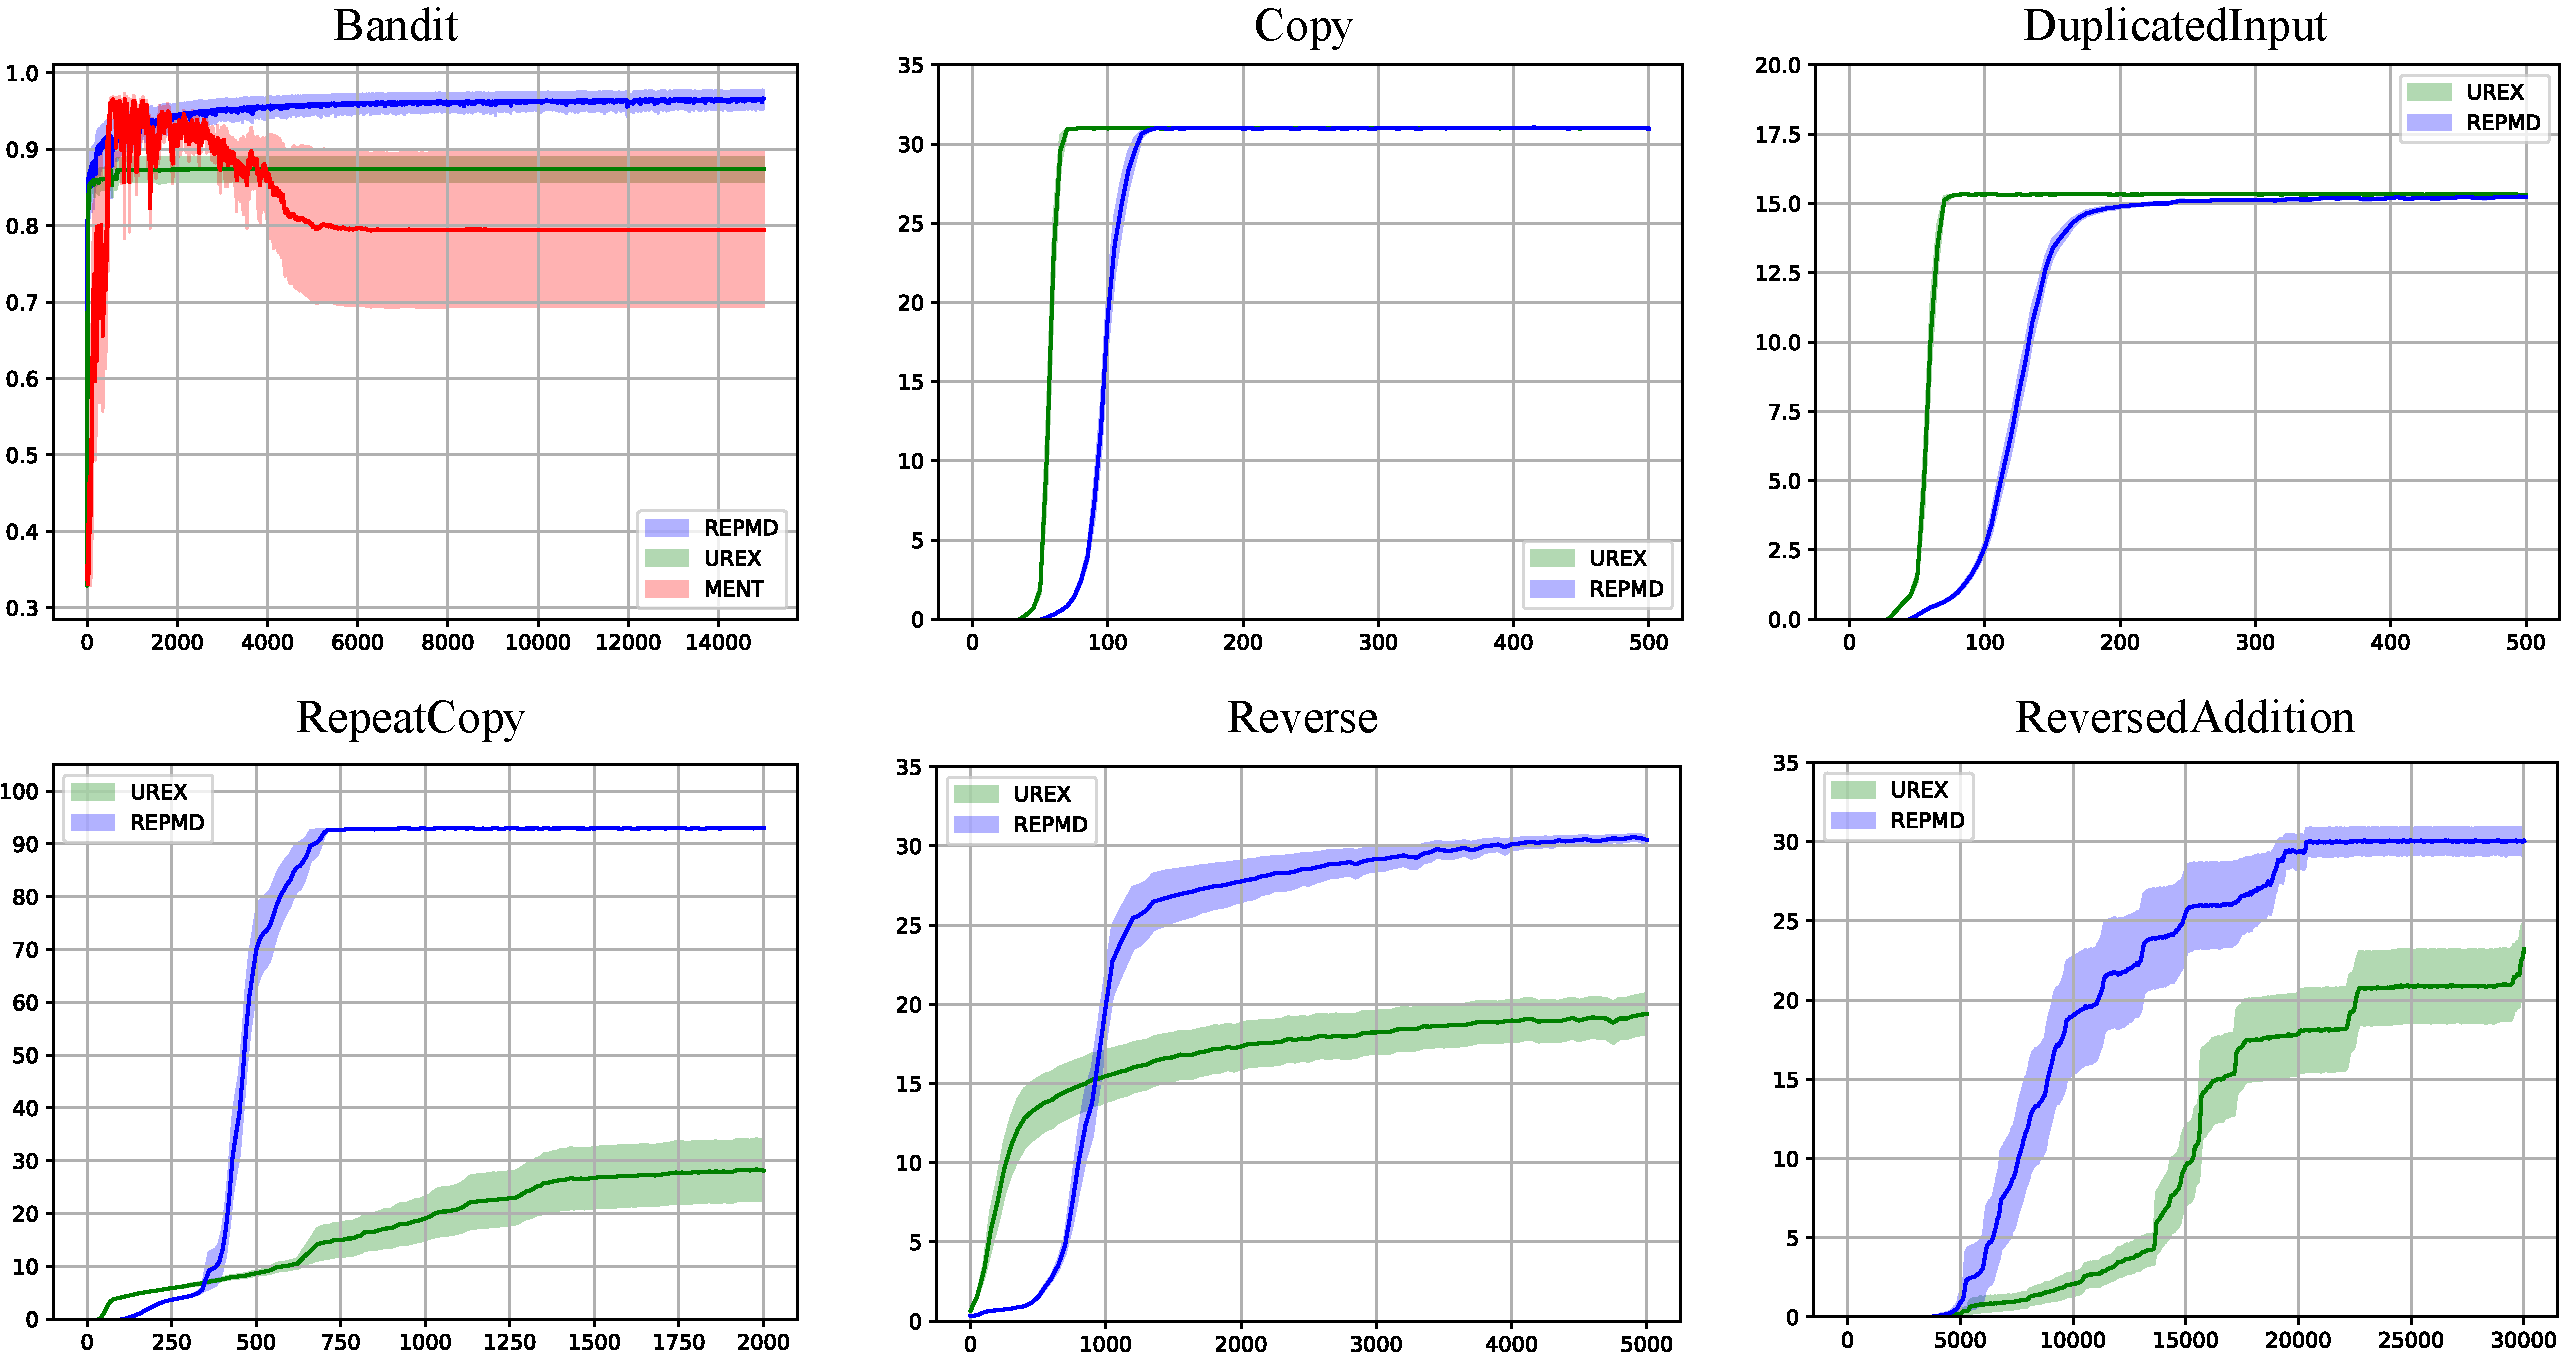
\includegraphics[width=0.85\linewidth]{./fig1.pdf}
\end{center}
\caption{
Results using the best hyper-parameters for each method: MENT (red), UREX (green), and REPMD (blue).
Plots show average reward with standard error during training. Synthetic bandit results averaged over 5 runs. Algorithmic task results averaged over 25 random training runs (5 runs $\times$ 5 random seeds for neural network initialization). X-axis is number of sampled trajectories. } 
\label{fig:results}
\end{figure*}

\subsection{Implementation Details}

For all of these algorithmic tasks, the policy is parameterized by a recurrent neural network with LSTM cells of hidden dimension 128 \citep{hochreiter1997long}. 

As shown in \cref{alg:repmd}, the policy is updated by performing KL divergence projection using stochastic gradient descent (SGD). In our experiments, the end condition of SGD is controlled by two parameters: $\epsilon > 0$ and $\text{F\_STEP}\in \{0,1 \}$. First, SGD halts if the change of the KL divergence is below or equal to $\epsilon$. Second, $\text{F\_STEP}$ decides the maximum number of SGD steps. If $\text{F\_STEP}=1$, the maximum number is $\sqrt{t}$ at iteration $t$; while if $\text{F\_STEP}=0$, there is no restriction on the maximum number of gradient steps, and stopping condition of SGD only depends on $\epsilon$.

For the synthetic bandit problem, we explore the following main hyper-parameters: learning rate $\eta \in \{0.1, 0.01, 0.001\}$; entropy regularizer of UREX and MENT $\tau\in \{1.0, 0.5, 0.1, 0.05\}$; relative entropy regularizer of REPMD $\tau\in \{1.0, 0.5, 0.1, 0.05\}$; $\epsilon\in \{0.01, 0.005, 0.001\}$ and $\text{F\_STEP}\in \{0,1\}$ for the stop condition of SGD in REPMD. The entropy regularizer $\tau'$ of REPMD is set to 0.  

For the algorithmic tasks, $N$ distinct environments are used to generate samples. On each environment, $K$ random trajectories are sampled using the agent's policy to estimate gradient according to (\ref{eq:gradient_estimator}), which gives the batch size $N\times K$ in total. We apply the same batch training setting as in UREX \citep{nachum2017improving}, where $N=40$ and $K=10$. The following main hyper-parameters are explored: learning rate $\eta \in \{0.1, 0.01, 0.001\}$; relative entropy regularizer of REPMD $\tau\in \{1.0, 0.5, 0.1, 0.05\}$; entropy regularizer of REPMD $\tau'\in \{0, 0.01, 0.005, 0.001\}$; gradient clipped norm for training LSTM $c\in \{1, 10, 40, 100\}$; $\epsilon\in \{0.01, 0.005, 0.001\}$ and $\text{F\_STEP}\in \{0,1\}$ for the stopping condition of SGD in REPMD. Parameters of UREX are set according to the ones reported in \citet{nachum2017improving}. Implementations of all algorithm are based on the open source code by the author of UREX \footnote{\url{https://github.com/tensorflow/models/tree/master/research/pcl_rl}}.

\subsection{Comparative Evaluation}

For the synthetic bandit problem, we compare REPMD against REINFORCE with entropy regularization (MENT) \citep{williams1992simple} and under-appreciated reward exploration (UREX) \citep{nachum2017improving}. For the algorithmic tasks, we compare REPMD only against UREX, since UREX has been shown to outperform MENT in these cases \citep{nachum2017improving}. The results are reported in Figure (\ref{fig:results}). It is clear that REPMD substantially outperforms the competitors on all of these benchmark tasks. REPMD is able to consistently achieve the highest score and learn substantially faster than UREX. We also find the performance of UREX is very unstable. On the difficult tasks, including RepeatCopy, Reverse and ReversedAddition, UREX can only successfully find appropriate solutions a few times out of 5 runs for each random seed, which brings the overall scores down. This observation creates the gap between our presented results with the ones reported in the paper\footnote{The results reported in \citet{nachum2017improving} averages over 5 runs of random restart, while our results are averaged over 25 random training runs (5 runs $\times$ 5 random seed for neural network initialization). }. Note that the performance of REPMD is sill significantly better than UREX even compared with the results reported in \citet{nachum2017improving}. 

%\begin{wrapfigure}{R}{0.5\textwidth}
%\label{fig:ablation}
%  \begin{center}
%    \includegraphics[width=0.5\textwidth]{Copy.png}
%  \end{center}
%  \caption{Hello, Bye!}
%\end{wrapfigure}

\subsection{Ablation Study}

\piccaption[]{Ablation Study.\label{fig:ablation}}
\parpic[r]{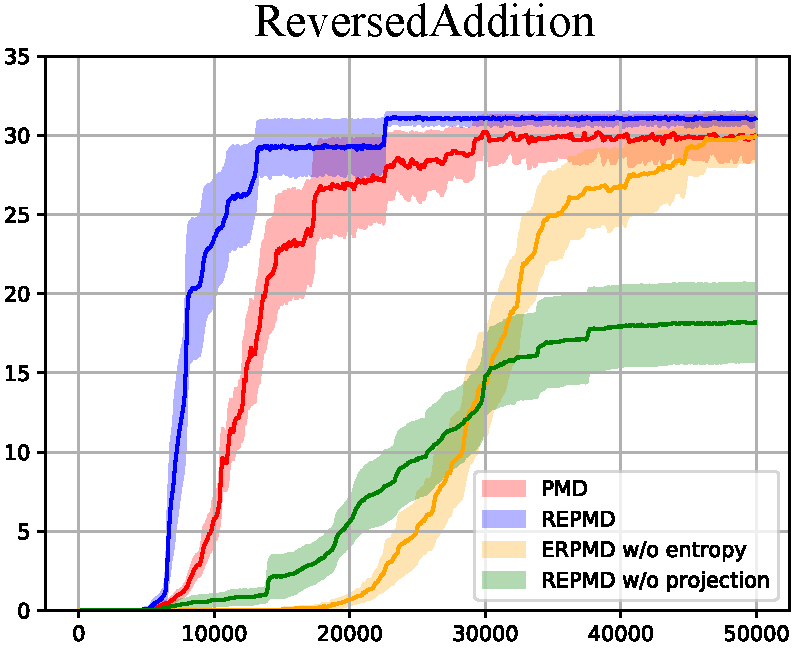
\includegraphics[width=0.35\linewidth]{ablation.pdf}}

\textbf{Importance of entropy regularizer.} The main difference between our objective \cref{eq:pmd} with the original MD is to add another entropy regularizer. We demonstrate the importance of this choice by presenting the results of REPMD with $\tau'=0$.

\textbf{Importance of KL divergence projection.} The main difference between REPMD and the UREX and MENT training methods is to use a projection step to optimize policy rather than performing a single gradient step. To show the importance of the projection step, we reimplement REPMD without projection, which only performs one step of gradient update at each iteration of training. 

\textbf{Importance of direction of KL divergence.} We implemented Policy Mirror Descent (PMD) as another baseline to prove the effectiveness of using the \emph{mean seeking} direction of KL divergence for policy optimization. Like in REPMD, we add a separate tempreture parameter $\tau'\geq 0$ to the original objective function (\ref{eq:max_expected_reward_plus_relative_entropy}) of PMD to encourage further exploration of the policy, which gives $\argmax_{\pi_\theta \in \Pi}{ \ep_{\rho \sim \pi_\theta}{  r(\rho)  - \tau \text{KL}(\pi_\theta \| \refPi) } + \tau'\cH(\pi_\theta) }$.

Results on ReversedAddition are reported in Figure (\ref{fig:ablation}). It clearly shows that optimizing policy by performing the \emph{mean seeking} KL divergence projection is very important as suggested in REPMD. 


\section{Conclusion and Future Work}
\label{sec:conclusion_and_future_work}

In this paper, we have proposed the reversed entropy policy mirror descent (REPMD) method for policy based reinforcement learning, which guarantees monotonic improvement in a well motivated objective. We show that the resulting method achieves better exploration than both a directed exploration method (UREX) and undirected maximum entropy exploration (MENT). It would be interesting to further extend the REPMD method within the actor-critic framework, by developing proper value function learning approach. %In particular, an actor-critic framework would also allow REPMD to perform important sampling on each step without heavy rollouts.


% \subsubsection*{Acknowledgments}

% Use unnumbered third level headings for the acknowledgments. All
% acknowledgments, including those to funding agencies, go at the end of the paper.

\bibliography{iclr2019_conference}
\bibliographystyle{iclr2019_conference}

\newpage
\appendix 
\section{Proof of \cref{thm:monotonically_increasing_sr_property}}
\begin{proof}
	Using $\KL(\bar{\pi}_{\tau,\tau^{\prime}}^* \| \pi_{\theta_{t+1}}) = \min_{\pi_\theta \in \Pi}{ \KL(\bar{\pi}_{\tau,\tau^{\prime}}^* \| \pi_\theta)} \le \KL(\bar{\pi}_{\tau,\tau^{\prime}}^* \| \pithetat)$ and Jensen's inequality,
	\begin{equation*}
	\begin{split}
	&\SR(\pi_{\theta_{t+1}}) - \SR(\pithetat) = (\tau + \tau^{\prime}) \log{ \sum\limits_{\rho}{ \frac{  \exp\left\{ \frac{r(\rho) + \tau \log{\pi_{\theta_{t+1}}(\rho)} }{\tau + \tau^{\prime}} \right\}  }{ \sum\limits_{\rho}{  \exp\left\{ \frac{r(\rho) + \tau \log{\pithetat(\rho)} }{\tau + \tau^{\prime}} \right\} } }  } } \\
	=& (\tau + \tau^{\prime}) \log{ \sum\limits_{\rho}{ \frac{  \exp\left\{ \frac{r(\rho) + \tau \log{\pithetat(\rho)} }{\tau + \tau^{\prime}} \right\}  }{ \sum\limits_{\rho}{  \exp\left\{ \frac{r(\rho) + \tau \log{\pithetat(\rho)} }{\tau + \tau^{\prime}} \right\} } }  } \cdot \exp\left\{ \frac{\tau \log{\pi_{\theta_{t+1}}(\rho)} - \tau \log{\pithetat(\rho)} }{\tau + \tau^{\prime}} \right\} } \\
	=& (\tau + \tau^{\prime}) \log{ \sum\limits_{\rho}{ \bar{\pi}_{\tau,\tau^{\prime}}^*(\rho) } \cdot \exp\left\{ \frac{\tau \log{\pi_{\theta_{t+1}}(\rho)} - \tau \log{\pithetat(\rho)} }{\tau + \tau^{\prime}} \right\} } \\
	\ge& (\tau + \tau^{\prime}) \sum\limits_{\rho}{ \bar{\pi}_{\tau,\tau^{\prime}}^*(\rho) \log{ \exp\left\{ \frac{\tau \log{\pi_{\theta_{t+1}}(\rho)} - \tau \log{\pithetat(\rho)} }{\tau + \tau^{\prime}} \right\} } } \\
	=& \tau \sum\limits_{\rho}{ \bar{\pi}_{\tau,\tau^{\prime}}^*(\rho) \log{ \frac{\pi_{\theta_{t+1}}(\rho)}{\pithetat(\rho)} } } = \tau \left[ \KL(\bar{\pi}_{\tau,\tau^{\prime}}^* \| \pithetat) - \KL(\bar{\pi}_{\tau,\tau^{\prime}}^* \| \pi_{\theta_{t+1}})\right] \ge 0. \qedhere
	\end{split}
	\end{equation*}
\end{proof}

\section{Stochastic Transition Setting}

In \cref{sec:notations_and_settings}, we assume that the state transition function is deterministic for simplicity. For completeness, we consider the general stochastic transition setting here.

\subsection{Notations and Settings}

Recall in \cref{sec:notations_and_settings}, the policy probability of trajectory $\rho=(s_1, a_1, \dots, a_{T-1}, s_T)$ is denoted as $\pi(\rho) = \prod_{t=1}^{T-1} \pi(a_t| s_t)$. We define transition probability of $\rho$ as $f(\rho) \triangleq \prod_{t=1}^{T-1}{ f(s_{s+1} | s_t, a_t)}$. The total probability of $\rho$ under policy $\pi$ and transition $f$ is then $p_{\pi, f}(\rho) \triangleq \pi(\rho) f(\rho) = \prod_{t=1}^{T-1}{ \pi(a_t | s_t) f(s_{s+1} | s_t, a_t)}$. We use $\Delta_{f} \triangleq \{ \pi | \sum_{\rho}{ p_{\pi, f}(\rho) } = \sum_{\rho}{\pi(\rho) f(\rho)} = 1, \pi(\rho) \ge 0, f(\rho) > 0, \forall \rho \}$ to refer to the probabilistic simplex over all possible trajectories. It is obvious that $p_{\pi, f}(\rho) = \pi(\rho)$ and $\Delta_f = \Delta$ under deterministic transition setting, i.e., $f(\rho) = 1, \forall \rho$.

\subsection{REPMD Optimization Problem}

The proposed REPMD algorithm solves \cref{eq:repmd} in the deterministic transition setting. In the stochastic setting, the corresponding problem is,
\begin{equation}
\label{eq:repmd_stochastic}
\begin{split}
	&\argmin\limits_{\pi_\theta \in \Pi}{\KL(p_{\bar{\pi}_{\tau,\tau^{\prime}}^*, f}  \| p_{\pi_\theta, f} ) }, \\
	\text{where}\ \ \bar{\pi}_{\tau,\tau^{\prime}}^* & =  \argmax\limits_{\pi \in \Delta_f}{ \ep\limits_{\rho \sim p_{\pi, f}}{ \left[ r(\rho) - \tau^{\prime} \log{\pi(\rho)} \right] } - \tau \KL(p_{\pi, f} \| p_{\pi_{\theta_t}, f} ) },
\end{split}
\end{equation}
which also recovers \cref{eq:repmd} as a special case when $f(\rho) = 1, \forall \rho$.

Like \cref{eq:repmd}, $\bar{\pi}_{\tau,\tau^{\prime}}^*$ in \cref{eq:repmd_stochastic} also has a closed form expression,
\begin{lem}
\label{lem:opt_pi_ref_stochastic}
The unconstrained optimal policy of \cref{eq:repmd_stochastic} has the following closed form expression:
\begin{equation*}
	\bar{\pi}_{\tau,\tau^{\prime}}^*(\rho) \triangleq \frac{\refPi(\rho) \exp\left\{ \frac{r(\rho)-\tau^{\prime} \log \refPi(\rho) }{ \tau+\tau^{\prime}} \right\}}{ \sum_{\rho^{\prime}}{\refPi(\rho^{\prime}) f(\rho^{\prime}) \exp\left\{ \frac{r(\rho^{\prime})-\tau^{\prime} \log \refPi(\rho^{\prime})}{ \tau+\tau^{\prime}} \right\} } }.
\end{equation*}
\end{lem}
\begin{proof}
Rewrite the maximization problem in \cref{eq:repmd_stochastic} as (take $\pi_{\theta_t}$ as the reference policy $\refPi$),
\begin{equation*}
\begin{split}
	\textmax\limits_{\pi}&{ \sum\limits_{\rho}{ \pi(\rho) f(\rho) \left[ r(\rho)  - \left( \tau + \tau^{\prime} \right) \log{\pi(\rho)} + \tau \log{\bar{\pi}(\rho)} \right]} } \\
	\st &\sum\limits_{\rho}{ \pi(\rho) f(\rho)} = 1.
\end{split}
\end{equation*}
The KKT condition of the above problem is,
\begin{equation*}
\begin{split}
	f(\rho) \left[ r(\rho) - \left( \tau + \tau^{\prime} \right) \log{\pi(\rho)} + \tau \log{\bar{\pi}(\rho)} +  \lambda - \left( \tau + \tau^{\prime} \right) \right] &= 0, \ \forall \rho \\
	\sum\limits_{\rho}{ \pi(\rho) f(\rho)} &= 1.
\end{split}
\end{equation*}
Using $f(\rho) > 0, \forall \rho$ and solving the KKT condition, we obtain the expression of $\bar{\pi}_{\tau,\tau^{\prime}}^*$.
\end{proof}

Lemma \ref{lem:opt_pi_ref_stochastic} recovers Lemma \ref{lem:opt_pi_ref} as a special case when $f(\rho) = 1, \forall \rho$.

\subsection{Theoretical Analysis}

In stochastic transition setting, we define the follow softmax approximated expected reward of $\pi_\theta$
\begin{equation*}
	\SR_f(\pi_\theta) \triangleq (\tau + \tau^{\prime})\log{ \sum_{\rho}{ f(\rho) \exp\left\{ \frac{r(\rho) + \tau \log{\pi_\theta(\rho)} }{\tau + \tau^{\prime}} \right\} }},
\end{equation*}
which recovers $\SR(\pi_\theta)$ when $f(\rho) = 1, \forall \rho$. The monotonic improvement property is for $\SR_f(\pi_\theta)$.

\begin{thm}
\label{thm:monotonically_increasing_sr_property_stochastic}
Assume that $\pi_{\theta_{t}}$ is the update sequence of the REPMD algorithm in \cref{eq:repmd_stochastic}, then
\begin{equation*}
	\SR_f(\pi_{\theta_{t+1}}) - \SR_f(\pithetat)\ge 0.
\end{equation*}
\end{thm}
\begin{proof}
	Using $\KL(p_{\bar{\pi}_{\tau,\tau^{\prime}}^*, f} \| p_{\pi_{\theta_{t+1}}, f}) = \min_{\pi_\theta \in \Pi}{ \KL(p_{\bar{\pi}_{\tau,\tau^{\prime}}^*, f}  \| p_{\pi_\theta, f} ) } \le \KL(p_{\bar{\pi}_{\tau,\tau^{\prime}}^*, f} \| p_{\pithetat, f})$ and Jensen's inequality,
	\begin{equation*}
	\begin{split}
	&\SR_f(\pi_{\theta_{t+1}}) - \SR_f(\pithetat) = (\tau + \tau^{\prime}) \log{ \sum\limits_{\rho}{ \frac{ f(\rho) \exp\left\{ \frac{r(\rho) + \tau \log{\pi_{\theta_{t+1}}(\rho)} }{\tau + \tau^{\prime}} \right\}  }{ \sum\limits_{\rho}{ f(\rho) \exp\left\{ \frac{r(\rho) + \tau \log{\pithetat(\rho)} }{\tau + \tau^{\prime}} \right\} } }  } } \\
	=& (\tau + \tau^{\prime}) \log{ \sum\limits_{\rho}{ \frac{ f(\rho) \exp\left\{ \frac{r(\rho) + \tau \log{\pithetat(\rho)} }{\tau + \tau^{\prime}} \right\}  }{ \sum\limits_{\rho}{ f(\rho) \exp\left\{ \frac{r(\rho) + \tau \log{\pithetat(\rho)} }{\tau + \tau^{\prime}} \right\} } }  } \cdot \exp\left\{ \frac{\tau \log{\pi_{\theta_{t+1}}(\rho)} - \tau \log{\pithetat(\rho)} }{\tau + \tau^{\prime}} \right\} } \\
	=& (\tau + \tau^{\prime}) \log{ \sum\limits_{\rho}{ \bar{\pi}_{\tau,\tau^{\prime}}^*(\rho) f(\rho) } \cdot \exp\left\{ \frac{\tau \log{\pi_{\theta_{t+1}}(\rho)} - \tau \log{\pithetat(\rho)} }{\tau + \tau^{\prime}} \right\} } \\
	\ge& (\tau + \tau^{\prime}) \sum\limits_{\rho}{ \bar{\pi}_{\tau,\tau^{\prime}}^*(\rho) f(\rho) \cdot \log{ \exp\left\{ \frac{\tau \log{\pi_{\theta_{t+1}}(\rho)} - \tau \log{\pithetat(\rho)} }{\tau + \tau^{\prime}} \right\} } } \\
	=& \tau \sum\limits_{\rho}{ \bar{\pi}_{\tau,\tau^{\prime}}^*(\rho) f(\rho) \cdot \log{ \frac{\pi_{\theta_{t+1}}(\rho)}{\pithetat(\rho)} } } \\
	=& \tau \sum\limits_{\rho}{ \bar{\pi}_{\tau,\tau^{\prime}}^*(\rho) f(\rho) \cdot \log{ \frac{ \pi_{\theta_{t+1}}(\rho) f(\rho) }{ \pithetat(\rho) f(\rho)} } } \\
	=& \tau \left[ \KL(p_{\bar{\pi}_{\tau,\tau^{\prime}}^*, f} \| p_{\pithetat, f}) - \KL(p_{\bar{\pi}_{\tau,\tau^{\prime}}^*, f} \| p_{\pi_{\theta_{t+1}}, f}) \right] \ge 0. \qedhere
	\end{split}
	\end{equation*}
\end{proof}

$\SR_f(\pi_\theta)$ also recovers corresponding performance measures in the stochastic transition setting.
\begin{prop}
\label{prop:sr_stochastic}
$\SR_f(\pi_\theta)$ satisfies the following properties:
\begin{enumerate}[label=(\roman*)]
	\item  $\SR_f(\pi_\theta) \to \max_{\rho}{r(\rho)}$, as $\tau \to 0, \tau^{\prime} \to 0$.
	\item $\SR_f(\pi_\theta) \to \ep\limits_{\rho \sim p_{\pi_\theta, f}}{r(\rho)}$, as $\tau \to \infty, \tau^{\prime} \to 0$. 
\end{enumerate}	
\end{prop}
\begin{proof}
To prove (i), note that as $\tau \to 0$, $\SR_f(\pi_\theta) \to \tau^{\prime} \log{ \sum_{\rho}{ f(\rho) \exp\left\{ \frac{r(\rho) }{ \tau^{\prime} } \right\} }}$. Taking limit on $\tau'$ gives the hardmax value $\max_{\rho}{r(\rho)}$ as $\tau^{\prime} \to 0$.
	
To prove (ii), we have 
\begin{align*}
	&\lim\limits_{\tau \to \infty}{ (\tau + \tau^{\prime})\log{ \sum_{\rho}{ f(\rho) \exp\left\{ \frac{r(\rho) + \tau \log{\pi_\theta(\rho)} }{\tau + \tau^{\prime}} \right\} }} } \\
	=& \lim\limits_{\tau \to \infty}{ \frac{ \sum_{\rho}{ \pi_\theta(\rho) f(\rho) \exp\{ \frac{r(\rho) - \tau^{\prime} \log{\pi_\theta(\rho)} }{\tau + \tau^{\prime}} \} \left( r(\rho) - \tau^{\prime}\log{\pi_\theta(\rho)} \right) } }{  \sum_{\rho}{ \pi_\theta(\rho) f(\rho) \exp\{ \frac{r(\rho) - \tau^{\prime} \log{\pi_\theta(\rho)} }{\tau + \tau^{\prime}} \} } } } \\
	=& \sum_{\rho}{ \pi_\theta(\rho) f(\rho) \left[ r(\rho) - \tau^{\prime}\log{\pi_\theta(\rho)} \right] } = \ep\limits_{\rho \sim p_{\pi_\theta, f}}{r(\rho)} -  \tau^{\prime} \cdot \ep\limits_{\rho \sim p_{\pi_\theta, f}}{  \log{\pi_\theta(\rho)} }
\end{align*}
As $\tau^{\prime} \to 0$, $\SR_f(\pi_\theta) \to \ep_{\rho \sim p_{\pi_\theta, f}}{r(\rho)}$.
\end{proof}

\subsection{Learning}

The REPMD learning process is intact under the stochastic transition setting. Similar with \cref{eq:importance_sampling_kl}, we can estimate the KL divergence in the projection step of \cref{eq:repmd_stochastic} by drawing $K$ \textit{i.i.d.} samples $\{\rho_1, \dots, \rho_K\}$ from $p_{\refPi, f}$, i.e., the mixture of $\refPi$ and $f$, which is exactly the process of sampling from $\refPi$ and interacting with the environment,
\begin{equation}
\label{eq:importance_sampling_kl_stochastic}
\begin{split}
	\KL(p_{\bar{\pi}_{\tau,\tau^{\prime}}^*, f}  \| p_{\pi_\theta, f} ) &= \ep_{\rho \sim p_{\bar{\pi}_{\tau,\tau^{\prime}}^*, f} } \left[ \log \bar{\pi}_{\tau,\tau^{\prime}}^*(\rho) - \log \pi_\theta(\rho) \right] \\
	&= \ep_{\rho\sim p_{\refPi, f}} \frac{\bar{\pi}_{\tau,\tau^{\prime}}^*(\rho)}{\refPi(\rho)} \left[ \log \bar{\pi}_{\tau,\tau^{\prime}}^*(\rho) - \log \pi_\theta(\rho) \right].
\end{split}
\end{equation}

We can then approximate the gradient of $\KL(p_{\bar{\pi}_{\tau,\tau^{\prime}}^*, f}  \| p_{\pi_\theta, f} )$ by averaging these $K$ samples according to \cref{eq:importance_sampling_kl_stochastic}. 

\begin{thm}
\label{thm:repmdgradientestimate_stochastic}
Let $\omega_k = \frac{r(\rho_k) - \tau^{\prime} \log{\refPi(\rho_k)} }{\tau + \tau^{\prime}}$. Given $K$ \emph{i.i.d.} samples $\{\rho_1, \dots, \rho_K\}$ from the \emph{reference policy} $\refPi$, we have the following unbiased gradient estimator,
\begin{equation}
	\nabla_{\theta} \KL(p_{\bar{\pi}_{\tau,\tau^{\prime}}^*, f}  \| p_{\pi_\theta, f} ) \approx -\sum\limits_{k=1}^K{ \frac{ \exp\left\{ \omega_k \right\} }{ \sum_{j=1}^K{ \exp\left\{ \omega_j \right\}}} \nabla_{\theta} \log{\pi_\theta(\rho_k)} },
\end{equation}
\end{thm}
\begin{proof}
See Theorem \ref{thm:repmdgradientestimate}.
\end{proof}

\end{document}
